% array4x4_max10.tex -- A 4x4 systolic array on Intel MAX 10: combinational and sequential logic,
% block by block and end to end.
% Build:  tectonic array4x4_max10.tex      (or: pdflatex array4x4_max10.tex, run twice)
\documentclass[aspectratio=169,11pt]{beamer}

\usepackage{tikz}
\usetikzlibrary{arrows.meta,positioning,shapes.geometric,calc,fit}
\usepackage{booktabs}
\usepackage{listings}
\usepackage{amsmath}
\usepackage{amssymb}
\usepackage{pifont}

% ---------------- look (same palette as the other decks) ----------------
\definecolor{pcb}{HTML}{0B2E33}
\definecolor{pcbmid}{HTML}{1F5C61}
\definecolor{tint}{HTML}{E6F0EF}
\definecolor{copper}{HTML}{B5651D}
\definecolor{coppert}{HTML}{F6E8DC}
\definecolor{ink}{HTML}{1F2A2E}
\definecolor{muted}{HTML}{5B6B70}
\definecolor{codebg}{HTML}{F4F7F7}
\definecolor{good}{HTML}{2E7D32}
\definecolor{bad}{HTML}{B3261E}
\definecolor{hardf}{HTML}{DCE6F2}
\definecolor{harde}{HTML}{2F4A7A}

\usetheme{default}
\setbeamercolor{background canvas}{bg=white}
\setbeamercolor{frametitle}{fg=pcb}
\setbeamercolor{normal text}{fg=ink}
\setbeamercolor{structure}{fg=pcbmid}
\setbeamerfont{frametitle}{series=\bfseries,size=\Large}
\setbeamertemplate{navigation symbols}{}
\setbeamertemplate{itemize item}{\color{copper}$\blacktriangleright$}
\setbeamertemplate{footline}{\hfill\color{muted}\scriptsize\insertframenumber\hspace{1.2em}\vspace{0.6em}}

\newcommand{\sig}[1]{\texttt{#1}}
\newcommand{\hx}[1]{\texttt{0x#1}}

\lstset{basicstyle=\ttfamily\fontsize{7.2}{8.6}\selectfont, backgroundcolor=\color{codebg},
  frame=single, rulecolor=\color{pcbmid}, keywordstyle=\color{pcbmid}\bfseries,
  commentstyle=\color{muted}\itshape, columns=fullflexible, keepspaces=true,
  morekeywords={logic,always_ff,signed,parameter,int,module,endmodule,input,output,assign,posedge,begin,end,if,else,for,genvar},
  xleftmargin=2pt, xrightmargin=2pt}

\tikzset{
  blk/.style  ={draw=pcbmid, fill=tint, rounded corners=3pt, thick, align=center,
                font=\footnotesize, inner sep=4pt},
  comb/.style ={draw=copper, fill=coppert, rounded corners=3pt, thick, align=center,
                font=\footnotesize, inner sep=3pt},
  seq/.style  ={draw=pcb, fill=white, very thick, align=center, font=\footnotesize, inner sep=3pt},
  hard/.style ={draw=harde, fill=hardf, thick, dashed, align=center, font=\footnotesize, inner sep=3pt},
  mix/.style  ={draw=pcbmid, fill=tint, rounded corners=3pt, thick, align=center,
                font=\footnotesize, inner sep=3pt},
  wires/.style={draw=muted, dashed, fill=white, align=center, font=\footnotesize, inner sep=3pt},
  wire/.style ={-{Stealth[length=2mm]}, thick, copper},
  wireb/.style={-{Stealth[length=2mm]}, thick, pcbmid},
  ctl/.style  ={-{Stealth[length=1.6mm]}, densely dashed, muted},
  w/.style    ={font=\scriptsize, text=muted, fill=white, inner sep=1pt},
  stn/.style  ={circle, fill=copper, text=white, inner sep=0.7pt, font=\tiny\bfseries},
}

% timing helpers: 1 cycle = \cw cm
\newcommand{\cw}{0.88}
\newcommand{\bus}[4]{% x0 x1 y text
  \draw[pcbmid] ({(#1)*\cw+0.06},#3) -- ({(#1)*\cw+0.12},#3+0.2) -- ({(#2)*\cw-0.06},#3+0.2) -- ({(#2)*\cw},#3)
                -- ({(#2)*\cw-0.06},#3-0.2) -- ({(#1)*\cw+0.12},#3-0.2) -- cycle;
  \node[font=\tiny\ttfamily] at ({((#1)+(#2))*\cw/2+0.03},#3) {#4};}
\newcommand{\pulse}[4]{% y, rise at cycle #2, fall at cycle #3, drawn up to cycle #4
  \draw[copper, thick] (0,#1-0.18) -- ({(#2)*\cw},#1-0.18) -- ({(#2)*\cw},#1+0.18) -- ({(#3)*\cw},#1+0.18)
                       -- ({(#3)*\cw},#1-0.18) -- ({(#4)*\cw},#1-0.18);}
\newcommand{\clockrow}[2]{% y, number of cycles
  \foreach \c in {1,...,#2} {
    \draw[pcbmid] ({(\c-1)*\cw},#1-0.18) -- ({(\c-1)*\cw},#1+0.18) -- ({(\c-0.5)*\cw},#1+0.18)
                  -- ({(\c-0.5)*\cw},#1-0.18) -- ({\c*\cw},#1-0.18);}}
% UART line: y (mm), list of 12 bit levels, cell width 9 mm
\newcommand{\uart}[2]{%
  \gdef\prev{1}%
  \foreach \l [count=\n from 0] in {#2} {
    \draw[copper, thick] (\n*9,#1+\l*5) -- (\n*9+9,#1+\l*5);
    \ifnum\l=\prev\relax\else\draw[copper, thick] (\n*9,#1) -- (\n*9,#1+5);\fi
    \global\let\prev\l
  }}

\title{\textcolor{pcb}{A 4$\times$4 Systolic Array on Intel MAX 10}}
\subtitle{Combinational and sequential logic, block by block and end to end}
\author{Deck 04 \textperiodcentered{} systolic-array project}
\date{}

\begin{document}

% =====================================================================
\begin{frame}
  \titlepage
  \centering\color{muted}\small
  Running design: \sig{N = 4}, \sig{K\_MAX = 64} (the Quartus build).
  Worked example: two 4$\times$4 matrices, K = 4.\\
  Numbers about the chip (LEs, critical path) are \textbf{estimates until Quartus compiles the design}.
\end{frame}

% =====================================================================
\begin{frame}{How to read this deck}
  \begin{columns}[T]
    \column{0.42\textwidth}
    \textbf{Colour code used in every figure}\\[2mm]
    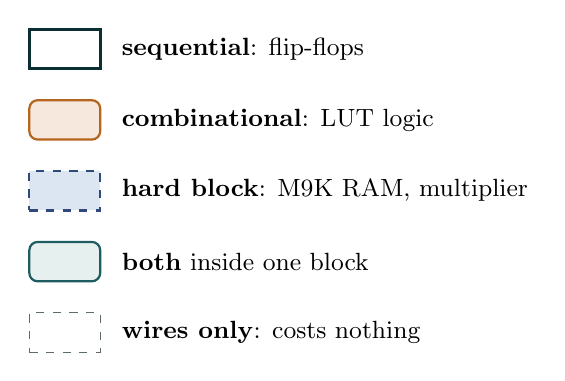
\begin{tikzpicture}[x=1mm,y=1mm]
      \node[seq,  minimum width=9mm, minimum height=5mm] at (0,0) {};
      \node[anchor=west, font=\small] at (6,0) {\textbf{sequential}: flip-flops};
      \node[comb, minimum width=9mm, minimum height=5mm] at (0,-9) {};
      \node[anchor=west, font=\small] at (6,-9) {\textbf{combinational}: LUT logic};
      \node[hard, minimum width=9mm, minimum height=5mm] at (0,-18) {};
      \node[anchor=west, font=\small] at (6,-18) {\textbf{hard block}: M9K RAM, multiplier};
      \node[mix,  minimum width=9mm, minimum height=5mm] at (0,-27) {};
      \node[anchor=west, font=\small] at (6,-27) {\textbf{both} inside one block};
      \node[wires, minimum width=9mm, minimum height=5mm] at (0,-36) {};
      \node[anchor=west, font=\small] at (6,-36) {\textbf{wires only}: costs nothing};
    \end{tikzpicture}
    \column{0.55\textwidth}\small
    \textbf{Parts}
    \begin{enumerate}
      \item The design we are building
      \item Combinational and sequential on MAX 10
      \item One PE on the chip
      \item Building the 4$\times$4 array
      \item Feeding the array: RAM, gate, skew
      \item Control: the FSM
      \item Time: one job, clock by clock
      \item Results and registers
      \item \textbf{End to end: follow one number}
      \item On the chip, and wrap-up
    \end{enumerate}
  \end{columns}
  \vspace{2mm}
  \begin{center}
  \colorbox{coppert}{\parbox{0.9\textwidth}{\centering\small The one rule behind every slide:
  \textbf{register $\rightarrow$ combinational logic $\rightarrow$ register}, once per clock (20\,ns at 50\,MHz).}}
  \end{center}
\end{frame}

% =====================================================================
\section{The design}
\begin{frame}{1.\ The job in numbers}
  \begin{columns}[T]
    \column{0.44\textwidth}\small
    \textbf{What one job computes}
    \[ \underbrace{C}_{4\times4,\ \text{int32}} \;=\; \underbrace{A}_{4\times K,\ \text{int8}} \cdot \underbrace{B}_{K\times4,\ \text{int8}} \]
    \centerline{\footnotesize with $1 \le K \le 64$}
    \textbf{Fixed hardware for N = 4}
    \begin{itemize}
      \item 16 PEs, so 16 multipliers and 16 accumulators
      \item 8 RAM banks (4 for A, 4 for B)
      \item 2 skew buffers, 1 controller FSM
      \item 1 register block with 5 performance counters
      \item 1 clock: 50\,MHz, 20\,ns per cycle
    \end{itemize}
    \column{0.53\textwidth}\small
    \textbf{Cost of one job}\\[1mm]
    \resizebox{\linewidth}{!}{%
\begin{tabular}{lrr}
      \toprule
       & \textbf{K = 4} & \textbf{K = 64} \\
      \midrule
      Cycles, START $\rightarrow$ DONE (K + 2N) & 12 & 72 \\
      Time at 50\,MHz & 240\,ns & 1.44\,$\mu$s \\
      MACs ($N^2K$) & 64 & 1\,024 \\
      PE utilization, $K/(K+2N-1)$ & 36.4\,\% & 90.1\,\% \\
      Throughput & 0.53\,GOPS & 1.42\,GOPS \\
      \bottomrule
    \end{tabular}}\\[2mm]
    Peak = $2 \times 16 \times 50\,\text{M}$ = \textbf{1.6\,GOPS}. Small K wastes most of the time filling and draining
    the array; large K gets close to the peak.
  \end{columns}
\end{frame}

% =====================================================================
\begin{frame}{2.\ The 4$\times$4 core: combinational vs sequential}
  \centering
  \resizebox{0.97\textwidth}{!}{%
  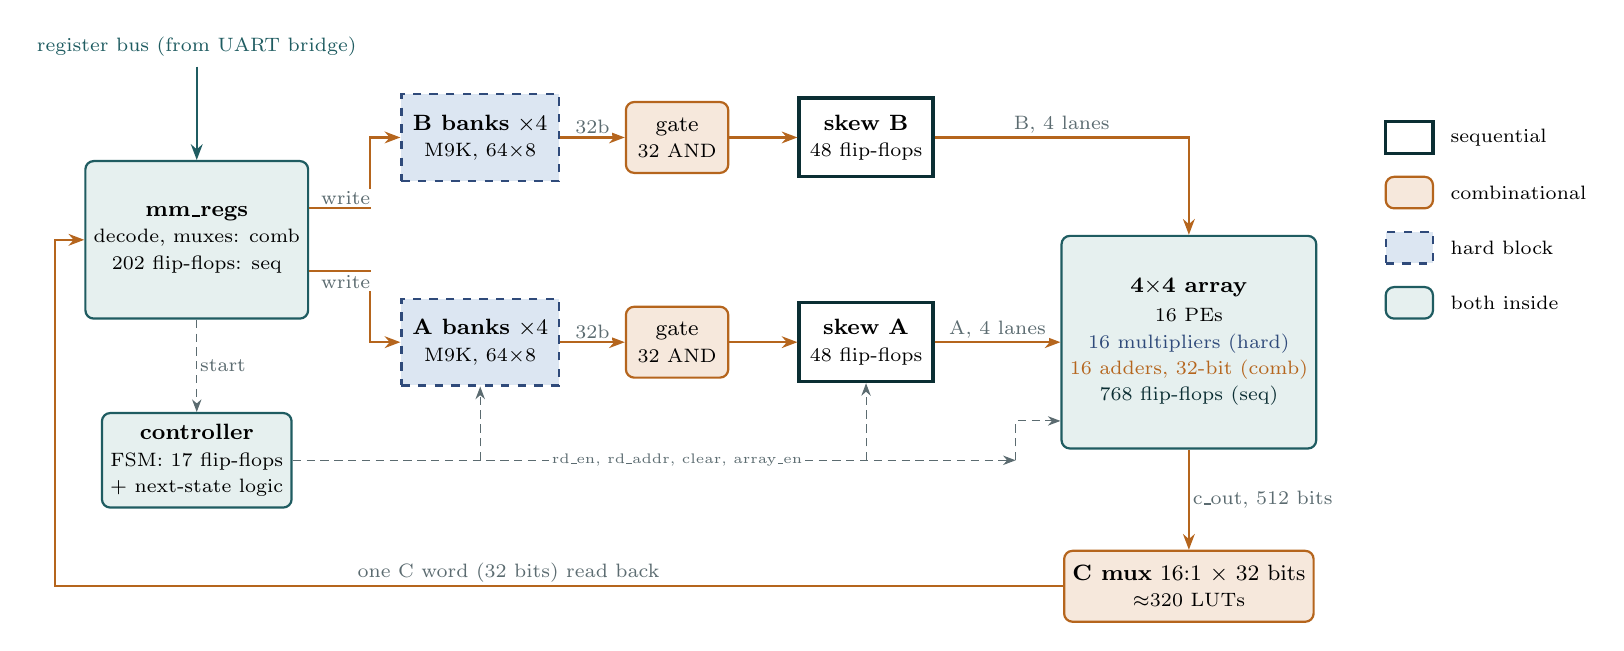
\begin{tikzpicture}[x=1mm,y=1mm]
    \node[mix, minimum width=24mm, minimum height=20mm] (regs) at (14,27)
      {\textbf{mm\_regs}\\\scriptsize decode, muxes: comb\\\scriptsize 202 flip-flops: seq};
    \node[mix, minimum width=24mm, minimum height=12mm] (ctrl) at (14,-1)
      {\textbf{controller}\\\scriptsize FSM: 17 flip-flops\\\scriptsize + next-state logic};
    \node[hard, minimum width=20mm, minimum height=11mm] (ab) at (50,14) {\textbf{A banks} $\times$4\\\scriptsize M9K, 64$\times$8};
    \node[hard, minimum width=20mm, minimum height=11mm] (bb) at (50,40) {\textbf{B banks} $\times$4\\\scriptsize M9K, 64$\times$8};
    \node[comb, minimum width=13mm, minimum height=9mm] (ga) at (75,14) {gate\\\scriptsize 32 AND};
    \node[comb, minimum width=13mm, minimum height=9mm] (gb) at (75,40) {gate\\\scriptsize 32 AND};
    \node[seq, minimum width=17mm, minimum height=10mm] (sa) at (99,14) {\textbf{skew A}\\\scriptsize 48 flip-flops};
    \node[seq, minimum width=17mm, minimum height=10mm] (sb) at (99,40) {\textbf{skew B}\\\scriptsize 48 flip-flops};
    \node[mix, minimum width=30mm, minimum height=27mm] (arr) at (140,14)
      {\textbf{4$\times$4 array}\\[1pt]\scriptsize 16 PEs\\\scriptsize\textcolor{harde}{16 multipliers (hard)}\\
       \scriptsize\textcolor{copper}{16 adders, 32-bit (comb)}\\\scriptsize\textcolor{pcb}{768 flip-flops (seq)}};
    \node[comb, minimum width=24mm, minimum height=9mm] (cm) at (140,-17) {\textbf{C mux} 16:1 $\times$ 32 bits\\\scriptsize $\approx$320 LUTs};
    \draw[wireb] (14,49) node[above, font=\scriptsize]{register bus (from UART bridge)} -- (regs.north);
    \draw[wire] (regs.east) ++(0,4) -| node[w,pos=0.3,above]{write} (36,40) -- (bb.west);
    \draw[wire] (regs.east) ++(0,-4) -| node[w,pos=0.3,below]{write} (36,14) -- (ab.west);
    \draw[wire] (ab) -- node[w,above]{32b} (ga);
    \draw[wire] (bb) -- node[w,above]{32b} (gb);
    \draw[wire] (ga) -- (sa);
    \draw[wire] (gb) -- (sb);
    \draw[wire] (sa) -- node[w,above]{A, 4 lanes} (arr.west);
    \draw[wire] (sb.east) -| node[w,pos=0.25,above]{B, 4 lanes} (arr.north);
    \draw[wire] (arr.south) -- node[w,right]{c\_out, 512 bits} (cm.north);
    \draw[wire] (cm.west) -- node[w,above,pos=0.55]{one C word (32 bits) read back} (-4,-17) |- (regs.west);
    \draw[ctl] (ctrl.east) -- (118,-1);
    \draw[ctl] (50,-1) -- (ab.south);
    \draw[ctl] (99,-1) -- (sa.south);
    \draw[ctl] (118,-1) -- (118,4) -- (arr.west |- 0,4);
    \node[font=\tiny, text=muted, fill=white, inner sep=1pt] at (75,-1) {rd\_en, rd\_addr, clear, array\_en};
    \draw[ctl] (regs.south) -- node[w,right]{start} (ctrl.north);
    \begin{scope}[shift={(168,40)}]
      \node[seq,  minimum width=6mm, minimum height=4mm] at (0,0) {};
      \node[anchor=west, font=\scriptsize] at (4,0) {sequential};
      \node[comb, minimum width=6mm, minimum height=4mm] at (0,-7) {};
      \node[anchor=west, font=\scriptsize] at (4,-7) {combinational};
      \node[hard, minimum width=6mm, minimum height=4mm] at (0,-14) {};
      \node[anchor=west, font=\scriptsize] at (4,-14) {hard block};
      \node[mix,  minimum width=6mm, minimum height=4mm] at (0,-21) {};
      \node[anchor=west, font=\scriptsize] at (4,-21) {both inside};
    \end{scope}
  \end{tikzpicture}}

  \vspace{1mm}\raggedright\footnotesize
  \begin{itemize}
    \item Data moves \textbf{one register stage per clock}: RAM $\rightarrow$ skew $\rightarrow$ PE $\rightarrow$ PE.
          The combinational parts sit \emph{between} registers and must settle within one 20\,ns clock period.
    \item Lane 0 of each skew buffer is a plain wire, so the likely longest path is
          \textbf{M9K $\rightarrow$ gate $\rightarrow$ PE(0,0) multiply + add $\rightarrow$ acc} (slide 31).
  \end{itemize}
\end{frame}

% =====================================================================
\begin{frame}[fragile]{3.\ Fifteen files become 44 hardware instances}
  \begin{columns}[T]
    \column{0.52\textwidth}
\begin{lstlisting}[basicstyle=\ttfamily\fontsize{6.6}{7.9}\selectfont]
top_de10lite              ports = physical pins
 +- u_key_sync : sync_2ff        buttons -> rst_n
 +- u_rx       : uart_rx         pin -> bytes
 |   +- u_sync : sync_2ff
 +- u_txq      : fifo_sync       bytes waiting to send
 +- u_tx       : uart_tx         bytes -> pin
 +- u_bridge   : uart_bus_bridge bytes <-> bus
 +- u_core     : mm_core         THE ACCELERATOR
 |   +- u_regs   : mm_regs       registers, counters
 |   +- u_ctrl   : mm_controller FSM
 |   +- g_bank[0..3].u_a : sram_sp   A banks
 |   +- g_bank[0..3].u_b : sram_sp   B banks
 |   +- u_skew_a, u_skew_b : skew_buffer
 |   +- u_array  : systolic_array
 |        +- g_row[i].g_col[j].u_pe : pe  (16)
 +- u_hb       : tick_gen        heartbeat LED
 +- g_digit[0..5].u_hex : hex7seg  HEX0-5
\end{lstlisting}
    \column{0.45\textwidth}\small
    \begin{itemize}
      \item Quartus gets \textbf{all 15 files} plus the name of the top: \sig{top\_de10lite}.
      \item It builds every instance with its parameters: N = 4 gives \textbf{16} \sig{pe} copies and
            \textbf{8} \sig{sram\_sp} copies.
      \item Then it \textbf{flattens} everything into one netlist of LUTs, flip-flops, multipliers and M9K blocks.
      \item Only the ports of \sig{top\_de10lite} get pins: clock, KEY, SW, LEDR, HEX, UART.
      \item Files talk only through \textbf{port connections}: a shared wire between two instances.
    \end{itemize}
  \end{columns}
\end{frame}

% =====================================================================
\section{Combinational and sequential}
\begin{frame}{4.\ Combinational vs sequential: the two kinds of logic}
  \begin{columns}[T]
    \column{0.48\textwidth}
    \textbf{Combinational}: output = f(inputs \emph{now})\\[1mm]
    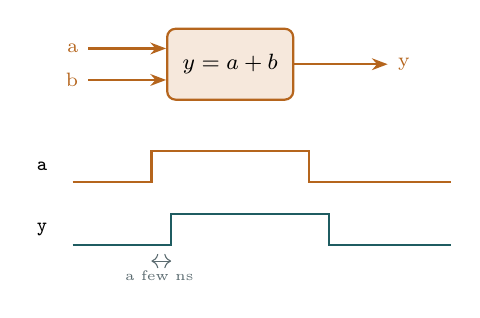
\begin{tikzpicture}[x=1mm,y=1mm]
      \node[comb, minimum width=16mm, minimum height=9mm] (g) at (24,0) {$y = a + b$};
      \draw[wire] (6,2) node[left,font=\scriptsize]{a} -- (g.west |- 0,2);
      \draw[wire] (6,-2) node[left,font=\scriptsize]{b} -- (g.west |- 0,-2);
      \draw[wire] (g.east) -- (44,0) node[right,font=\scriptsize]{y};
      \node[font=\scriptsize\ttfamily, anchor=east] at (2,-13) {a};
      \node[font=\scriptsize\ttfamily, anchor=east] at (2,-21) {y};
      \draw[copper, thick] (4,-15) -- (14,-15) -- (14,-11) -- (34,-11) -- (34,-15) -- (52,-15);
      \draw[pcbmid, thick] (4,-23) -- (16.5,-23) -- (16.5,-19) -- (36.5,-19) -- (36.5,-23) -- (52,-23);
      \draw[muted, <->] (14,-25) -- (16.5,-25);
      \node[font=\tiny, text=muted, anchor=north] at (15,-25) {a few ns};
    \end{tikzpicture}\\
    \footnotesize No clock, no memory. The output follows the inputs after a small delay.
    In our design: multipliers, adders, decoders, multiplexers.
    \column{0.48\textwidth}
    \textbf{Sequential}: output changes only at the clock edge\\[1mm]
    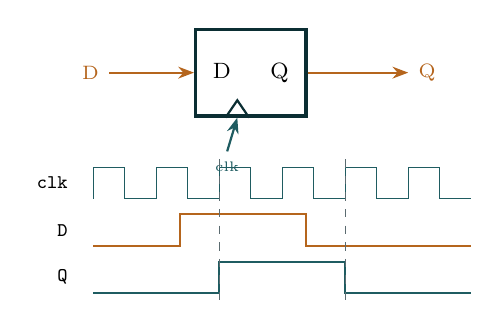
\begin{tikzpicture}[x=1mm,y=1mm]
      \node[seq, minimum width=14mm, minimum height=11mm] (ff) at (24,0) {D \hspace{3mm} Q};
      \draw[pcb, thick] ($(ff.south west)+(4,0)$) -- ++(1.5,2.2) -- ++(1.5,-2.2);
      \draw[wire] (6,0) node[left,font=\scriptsize]{D} -- (ff.west);
      \draw[wire] (ff.east) -- (44,0) node[right,font=\scriptsize]{Q};
      \draw[wireb] (21,-10) node[below,font=\tiny]{clk} -- ($(ff.south west)+(5.5,0)$);
      \foreach \y/\s in {-14/clk, -20/D, -26/Q} \node[font=\scriptsize\ttfamily, anchor=east] at (2,\y) {\s};
      \foreach \e in {0,1,2,3,4,5} \draw[pcbmid] (4+\e*8,-16) -- (4+\e*8,-12) -- (8+\e*8,-12) -- (8+\e*8,-16) -- (12+\e*8,-16);
      \draw[copper, thick] (4,-22) -- (15,-22) -- (15,-18) -- (31,-18) -- (31,-22) -- (52,-22);
      \draw[pcbmid, thick] (4,-28) -- (20,-28) -- (20,-24) -- (36,-24) -- (36,-28) -- (52,-28);
      \foreach \x in {20,36} \draw[muted, dashed] (\x,-11) -- (\x,-29);
    \end{tikzpicture}\\
    \footnotesize Q copies D \textbf{only at a rising edge} and holds it until the next one.
    In our design: \sig{acc}, \sig{a\_out}, skew registers, FSM state, counters.
  \end{columns}
  \vspace{1mm}
  \centering
  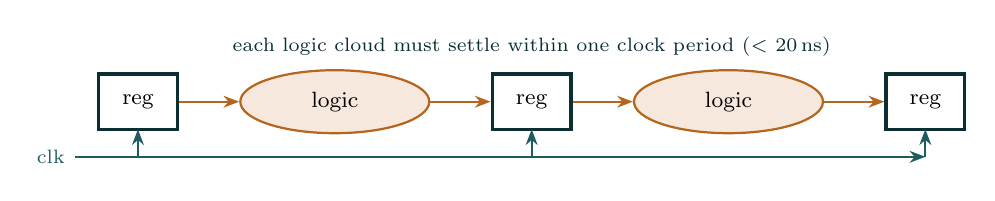
\begin{tikzpicture}[x=1mm,y=1mm]
    \node[seq, minimum width=10mm, minimum height=7mm] (r1) at (0,0) {reg};
    \node[comb, ellipse, minimum width=24mm, minimum height=8mm] (c1) at (25,0) {logic};
    \node[seq, minimum width=10mm, minimum height=7mm] (r2) at (50,0) {reg};
    \node[comb, ellipse, minimum width=24mm, minimum height=8mm] (c2) at (75,0) {logic};
    \node[seq, minimum width=10mm, minimum height=7mm] (r3) at (100,0) {reg};
    \draw[wire] (r1) -- (c1); \draw[wire] (c1) -- (r2); \draw[wire] (r2) -- (c2); \draw[wire] (c2) -- (r3);
    \draw[wireb] (-8,-7) node[left,font=\scriptsize]{clk} -- (100,-7);
    \foreach \x in {0,50,100} \draw[wireb] (\x,-7) -- (\x,-3.5);
    \node[font=\scriptsize, text=pcb] at (50,7) {each logic cloud must settle within one clock period ($<$ 20\,ns)};
  \end{tikzpicture}
\end{frame}

% =====================================================================
\begin{frame}{5.\ What each kind of logic becomes on MAX 10}
  \small
  \resizebox{\textwidth}{!}{%
\begin{tabular}{@{}llll@{}}
    \toprule
    \textbf{In the RTL} & \textbf{Kind} & \textbf{On the MAX 10 chip} & \textbf{In our 4$\times$4} \\
    \midrule
    \sig{always\_ff} register & sequential & LE flip-flop & PE regs, skew, FSM, counters \\
    \sig{+}, \sig{==}, counters & combinational & LUTs + fast carry chain & 16 adders (32-bit), counters \\
    \sig{case}, \sig{?:}, \sig{\&\&} & combinational & 4-input LUTs & decode, muxes, FSM logic \\
    \sig{*} (8$\times$8 signed) & combinational & 9$\times$9 embedded multiplier & 16 of 288 \\
    \sig{mem[addr]} in \sig{always\_ff} & sequential & M9K block RAM & 8 of 182 \\
    sign extension, bit slices & --- & wires only, 0 LEs & \sig{AW'(prod)}, \sig{offset[11:6]} \\
    \bottomrule
  \end{tabular}}
  \vspace{4mm}
  \begin{itemize}
    \item \textbf{LE} (logic element) = one 4-input LUT + carry logic + one flip-flop. The 10M50 has \textbf{49\,760} LEs.
    \item \textbf{M9K} = 9\,216-bit RAM block. Its address is \textbf{registered}, so data comes out one clock after the
          address goes in. That one clock shows up everywhere in our timing.
    \item MAX 10 has \textbf{no LUT-RAM}: small memories (like the 16-byte UART FIFO) become flip-flops.
  \end{itemize}
\end{frame}

% =====================================================================
\begin{frame}{6.\ Inside the chip: the logic element (LE) and the LAB}
  \centering
  \resizebox{0.96\textwidth}{!}{%
  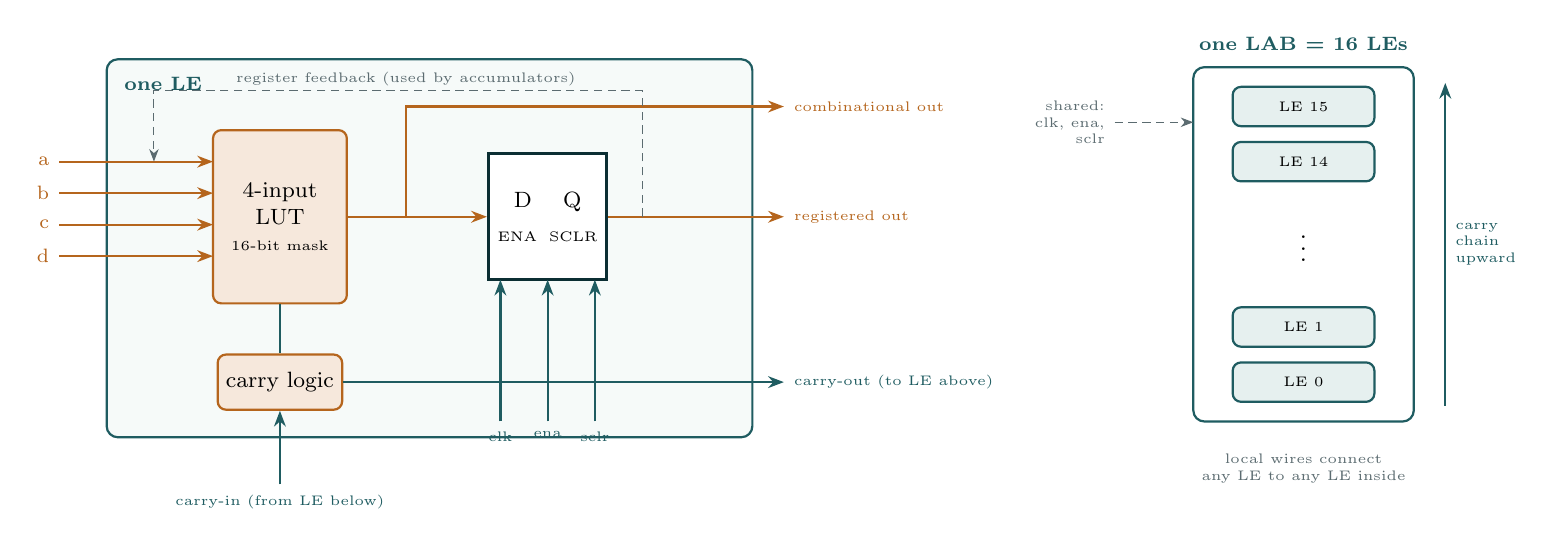
\begin{tikzpicture}[x=1mm,y=1mm]
    \draw[pcbmid, rounded corners, thick, fill=tint!35] (-2,-10) rectangle (80,38);
    \node[font=\scriptsize\bfseries, text=pcbmid, anchor=north west] at (-1,37) {one LE};
    \node[comb, minimum width=17mm, minimum height=22mm] (lut) at (20,18) {4-input\\LUT\\\tiny 16-bit mask};
    \foreach \y/\s in {25/a, 21/b, 17/c, 13/d} \draw[wire] (-8,\y) node[left,font=\scriptsize]{\s} -- (11.5,\y);
    \node[comb, minimum width=15mm, minimum height=7mm] (cy) at (20,-3) {carry logic};
    \draw[wireb] (20,-16) node[below,font=\tiny]{carry-in (from LE below)} -- (cy.south);
    \draw[wireb] (cy.east) -- (84,-3) node[right,font=\tiny]{carry-out (to LE above)};
    \draw[pcbmid, thick] (lut.south) -- (cy.north);
    \node[seq, minimum width=15mm, minimum height=16mm] (ff) at (54,18) {D\hspace{4mm}Q\\[3pt]\tiny ENA\; SCLR};
    \draw[wire] (lut.east) -- (ff.west);
    \draw[wire] (36,18) |- (84,32) node[right,font=\tiny]{combinational out};
    \draw[wire] (ff.east) -- (84,18) node[right,font=\tiny]{registered out};
    \draw[ctl] (66,18) |- (4,34) -- (4,25);
    \node[font=\tiny, text=muted, fill=tint!35, inner sep=1pt] at (36,35.5) {register feedback (used by accumulators)};
    \foreach \x/\s in {48/clk, 54/ena, 60/sclr} \draw[wireb] (\x,-8) node[below,font=\tiny]{\s} -- (\x,10);
    % LAB
    \begin{scope}[shift={(150,0)}]
      \foreach \k/\y in {15/32, 14/25, 1/4, 0/-3} \node[blk, minimum width=18mm, minimum height=5mm, font=\tiny] at (0,\y) {LE \k};
      \node[font=\small] at (0,15) {$\vdots$};
      \draw[pcbmid, rounded corners, thick] (-14,-8) rectangle (14,37);
      \node[font=\scriptsize\bfseries, text=pcbmid] at (0,40) {one LAB = 16 LEs};
      \draw[wireb] (18,-6) -- (18,35) node[right,font=\tiny, align=left, pos=0.5]{carry\\chain\\upward};
      \draw[ctl] (-24,30) node[left, font=\tiny, align=right]{shared:\\clk, ena,\\sclr} -- (-14,30);
      \node[font=\tiny, text=muted, align=center] at (0,-14) {local wires connect\\any LE to any LE inside};
    \end{scope}
  \end{tikzpicture}}

  \vspace{1mm}\raggedright\footnotesize
  \begin{itemize}
    \item \textbf{Normal mode}: the LUT is any 4-input function (decoders, muxes, FSM logic).
          \textbf{Arithmetic mode}: it splits into a \emph{sum} LUT and a \emph{carry} LUT, one adder bit per LE.
    \item The 16 LEs of a LAB share their clock, clock-enable and clear. All PE registers use the same three
          (\sig{clk}, \sig{en}, \sig{!rst\_n || clear}), so they pack neatly. 10M50: 3\,110 LABs.
  \end{itemize}
\end{frame}

% =====================================================================
\begin{frame}{7.\ Clock, reset, clear and enable: the signals every register sees}
  \begin{columns}[T]
    \column{0.58\textwidth}
    \centering
    \resizebox{\linewidth}{!}{%
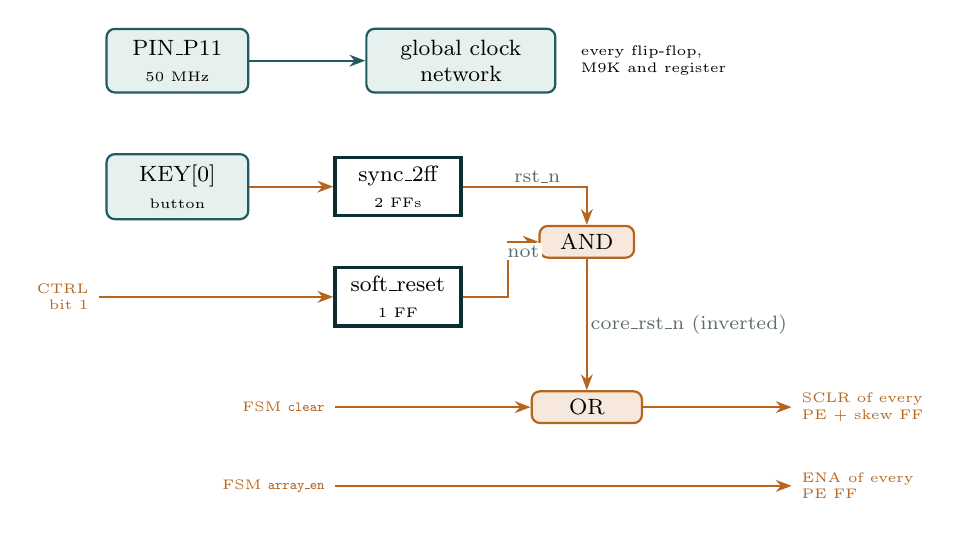
\begin{tikzpicture}[x=1mm,y=1mm]
      \node[blk, minimum width=18mm] (pin) at (0,30) {PIN\_P11\\\tiny 50 MHz};
      \node[blk, minimum width=24mm] (gclk) at (36,30) {global clock\\network};
      \node[font=\tiny, align=left, anchor=west] at (50,30) {every flip-flop,\\M9K and register};
      \draw[wireb] (pin) -- (gclk);
      \node[blk, minimum width=18mm] (key) at (0,14) {KEY[0]\\\tiny button};
      \node[seq, minimum width=16mm] (sy) at (28,14) {sync\_2ff\\\tiny 2 FFs};
      \node[seq, minimum width=16mm] (sr) at (28,0) {soft\_reset\\\tiny 1 FF};
      \node[comb, minimum width=12mm] (and) at (52,7) {AND};
      \draw[wire] (key) -- (sy);
      \draw[wire] (sy) -| node[w,pos=0.3,above]{rst\_n} (and.north);
      \draw[wire] (sr.east) -- (42,0) |- node[w,pos=0.75,below]{not} (and.west);
      \draw[wire] (-10,0) node[left,font=\tiny,align=right]{CTRL\\bit 1} -- (sr);
      \node[comb, minimum width=14mm] (or) at (52,-14) {OR};
      \draw[wire] (and.south) -- node[w,right]{core\_rst\_n (inverted)} (or.north);
      \draw[wire] (20,-14) node[left,font=\tiny]{FSM \sig{clear}} -- (or.west);
      \draw[wire] (or.east) -- (78,-14) node[right,font=\tiny,align=left]{SCLR of every\\PE + skew FF};
      \draw[wire] (20,-24) node[left,font=\tiny]{FSM \sig{array\_en}} -- (78,-24) node[right,font=\tiny,align=left]{ENA of every\\PE FF};
    \end{tikzpicture}}
    \column{0.40\textwidth}\small
    \begin{itemize}
      \item \textbf{One clock}, 50\,MHz, on the chip's global clock network. One clock domain, so no CDC except
            the asynchronous inputs (button, UART RX), which go through \sig{sync\_2ff}.
      \item \textbf{Synchronous} reset: nothing happens between edges.
      \item In every PE:\\[1mm]
      {\ttfamily\scriptsize if (!rst\_n || clear) zero\\
       else if (en) update\\
       else hold}\\[1mm]
      becomes SCLR and ENA on the flip-flops: almost no extra logic.
    \end{itemize}
  \end{columns}
\end{frame}

% =====================================================================
\section{One PE}
\begin{frame}{8.\ One PE: the combinational part and the sequential part}
  \centering
  \resizebox{0.9\textwidth}{!}{%
  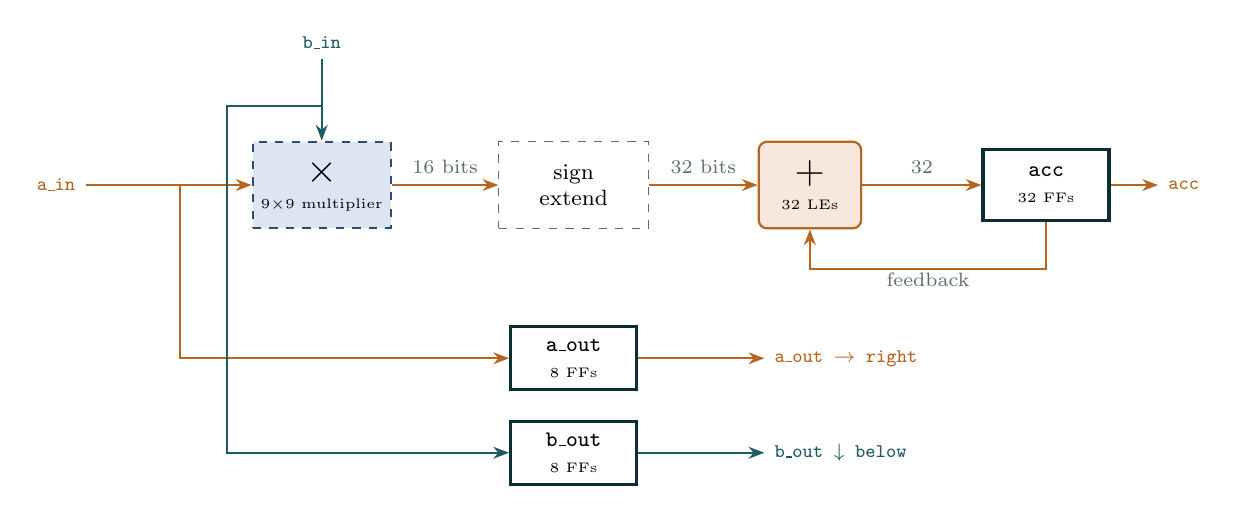
\begin{tikzpicture}[x=1mm,y=1mm]
    \node[hard, minimum width=17mm, minimum height=11mm] (mul) at (30,20) {\Large$\times$\\\tiny 9$\times$9 multiplier};
    \node[wires, minimum width=19mm, minimum height=11mm] (ext) at (62,20) {sign\\extend};
    \node[comb, minimum width=13mm, minimum height=11mm] (add) at (92,20) {\Large$+$\\\tiny 32 LEs};
    \node[seq, minimum width=16mm, minimum height=9mm] (acc) at (122,20) {\sig{acc}\\\tiny 32 FFs};
    \node[seq, minimum width=16mm, minimum height=8mm] (ar) at (62,-2) {\sig{a\_out}\\\tiny 8 FFs};
    \node[seq, minimum width=16mm, minimum height=8mm] (br) at (62,-14) {\sig{b\_out}\\\tiny 8 FFs};
    \draw[wire] (0,20) node[left,font=\scriptsize\ttfamily]{a\_in} -- (mul.west);
    \draw[wireb] (30,36) node[above,font=\scriptsize\ttfamily]{b\_in} -- (mul.north);
    \draw[wire] (mul) -- node[w,above=1mm]{16 bits} (ext);
    \draw[wire] (ext) -- node[w,above=1mm]{32 bits} (add);
    \draw[wire] (add) -- node[w,above=1mm]{32} (acc);
    \draw[wire] (acc.east) -- ++(6,0) node[right,font=\scriptsize\ttfamily]{acc};
    \draw[wire] (acc.south) -- ++(0,-6) -| (add.south);
    \node[w] at (107,8) {feedback};
    \draw[wire] (12,20) |- (ar.west);
    \draw[wireb] (30,30) -| (18,-14) -- (br.west);
    \draw[wire] (ar.east) -- ++(16,0) node[right,font=\scriptsize\ttfamily]{a\_out $\rightarrow$ right};
    \draw[wireb] (br.east) -- ++(16,0) node[right,font=\scriptsize\ttfamily]{b\_out $\downarrow$ below};
  \end{tikzpicture}}

  \vspace{1mm}\raggedright\small
  \begin{itemize}
    \item \textbf{Combinational} (settles during the cycle): multiply (hard block), sign extension (wires only),
          32-bit add (LUTs + carry chain).
    \item \textbf{Sequential} (changes at the edge): \sig{acc}, \sig{a\_out}, \sig{b\_out} = 32 + 8 + 8 = \textbf{48 flip-flops}.
    \item On MAX 10: \textbf{1} multiplier + \textbf{32} LEs that hold an adder bit \emph{and} an \sig{acc} bit + \textbf{16} LEs
          used only for their flip-flop.
  \end{itemize}
\end{frame}

% =====================================================================
\begin{frame}{9.\ One accumulator bit = one LE in arithmetic mode}
  \begin{columns}[T]
    \column{0.47\textwidth}
    \centering
    \resizebox{\linewidth}{!}{%
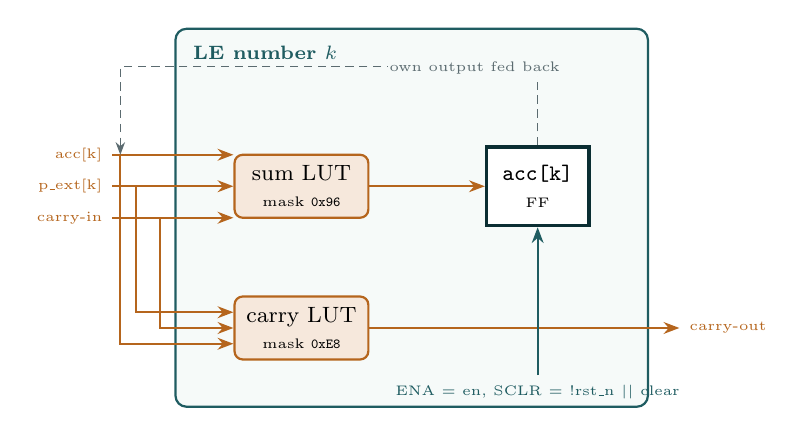
\begin{tikzpicture}[x=1mm,y=1mm]
      \draw[pcbmid, rounded corners, thick, fill=tint!35] (-4,-14) rectangle (56,34);
      \node[font=\scriptsize\bfseries, text=pcbmid, anchor=north west] at (-3,33) {LE number $k$};
      \node[comb, minimum width=17mm, minimum height=8mm] (s) at (12,14) {sum LUT\\\tiny mask \hx{96}};
      \node[comb, minimum width=17mm, minimum height=8mm] (c) at (12,-4) {carry LUT\\\tiny mask \hx{E8}};
      \node[seq, minimum width=13mm, minimum height=10mm] (ff) at (42,14) {\sig{acc[k]}\\\tiny FF};
      \draw[wire] (s) -- (ff);
      \draw[wire] (-12,18) node[left,font=\tiny]{acc[k]} -- (s.west |- 0,18);
      \draw[wire] (-12,14) node[left,font=\tiny]{p\_ext[k]} -- (s.west);
      \draw[wire] (-12,10) node[left,font=\tiny]{carry-in} -- (s.west |- 0,10);
      \draw[wire] (-6,10) |- (c.west);
      \draw[wire] (-9,14) |- ($(c.west)+(0,2)$);
      \draw[wire] (-11,18) |- ($(c.west)+(0,-2)$);
      \draw[wire] (c.east) -- (60,-4) node[right,font=\tiny]{carry-out};
      \draw[ctl] (ff.north) -- ++(0,10) -| (-11,22) -- (-11,18);
      \node[font=\tiny, text=muted, fill=tint!35, inner sep=0.5pt] at (34,29) {own output fed back};
      \draw[wireb] (42,-10) node[below,font=\tiny]{ENA = en, SCLR = !rst\_n $\vert\vert$ clear} -- (ff.south);
    \end{tikzpicture}}\\[1mm]
    \footnotesize sum = a $\oplus$ b $\oplus$ cin (truth table \sig{01101001} = \hx{96});
    carry = majority (\sig{00010111} = \hx{E8}). 32 of these LEs in a chain = one PE accumulator (2 LABs).
    \column{0.5\textwidth}\small
    \textbf{Real numbers: PE(1,2) at step t = 5}\\
    acc = 4, product = $-1$, so p\_ext = \hx{FFFFFFFF}.\\[1mm]
    \begin{tabular}{@{}lccccc@{}}
      \toprule
      LE (bit) & a = acc & b = p & cin & \textbf{sum} & cout \\
      \midrule
      0 & 0 & 1 & 0 & \textbf{1} & 0 \\
      1 & 0 & 1 & 0 & \textbf{1} & 0 \\
      2 & 1 & 1 & 0 & \textbf{0} & 1 \\
      3 & 0 & 1 & 1 & \textbf{0} & 1 \\
      4 \ldots 31 & 0 & 1 & 1 & \textbf{0} & 1 \\
      \bottomrule
    \end{tabular}\\[2mm]
    The carry out of bit 31 is dropped. Result \hx{00000003} = \textbf{3} = $4 + (-1)$ \checkmark\\[1mm]
    The \textbf{carry ripples} through 32 LEs during the cycle (combinational); the 32 flip-flops take the new value
    at the edge (sequential).
  \end{columns}
\end{frame}

% =====================================================================
\section{The array}
\begin{frame}{10.\ Wiring 16 PEs: only wires between them}
  \begin{columns}[T]
    \column{0.55\textwidth}
    \centering
    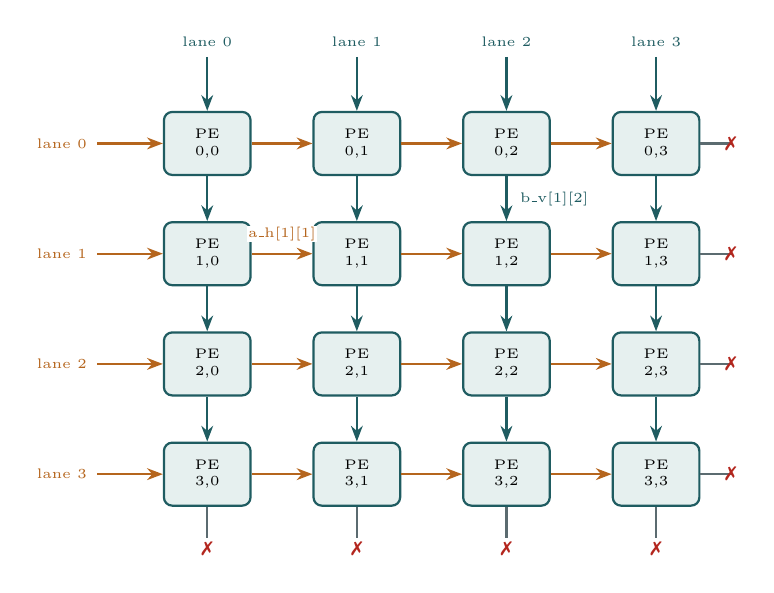
\begin{tikzpicture}[x=1mm,y=1mm]
      \foreach \i in {0,...,3} \foreach \j in {0,...,3}
        \node[mix, minimum width=11mm, minimum height=8mm, inner sep=0pt, font=\tiny] (p\i\j) at (\j*19,-\i*14) {PE\\\i,\j};
      \foreach \i in {0,...,3} \foreach \j/\jn in {0/1,1/2,2/3} \draw[wire] (p\i\j) -- (p\i\jn);
      \foreach \j in {0,...,3} \foreach \i/\inn in {0/1,1/2,2/3} \draw[wireb] (p\i\j) -- (p\inn\j);
      \foreach \i in {0,...,3} \draw[wire] (-14,-\i*14) node[left,font=\tiny]{lane \i} -- (p\i0);
      \foreach \j in {0,...,3} \draw[wireb] (\j*19,11) node[above,font=\tiny]{lane \j} -- (p0\j);
      \foreach \i in {0,...,3} {\draw[muted, thick] (p\i3.east) -- ++(4,0); \node[text=bad, font=\scriptsize] at (66.5,-\i*14) {\ding{55}};}
      \foreach \j in {0,...,3} {\draw[muted, thick] (p3\j.south) -- ++(0,-4); \node[text=bad, font=\scriptsize] at (\j*19,-51.5) {\ding{55}};}
      \node[font=\tiny, text=copper, fill=white, inner sep=0.5pt] at (9.5,-11.5) {a\_h[1][1]};
      \node[font=\tiny, text=pcbmid, fill=white, inner sep=0.5pt, anchor=west] at (39.5,-7) {b\_v[1][2]};
    \end{tikzpicture}
    \column{0.43\textwidth}\small
    \begin{itemize}
      \item Each arrow is one 8-bit wire, for example \sig{a\_h[1][1]}: it is PE(1,0)'s \sig{a\_out} \textbf{and}
            PE(1,1)'s \sig{a\_in}.
      \item There is \textbf{no logic between PEs}. Every PE-to-PE path is register (\sig{a\_out}) $\rightarrow$
            multiply + add in the next PE $\rightarrow$ register (\sig{acc}).
      \item \textcolor{bad}{\ding{55}} The last column's \sig{a\_out} and the bottom row's \sig{b\_out} drive nothing.
            Quartus removes them: $8 \times 8 = 64$ flip-flops, so \textbf{704} of the 768 remain (expected).
      \item All 16 PEs share \sig{clk}, \sig{rst\_n}, \sig{clear} and \sig{en}.
    \end{itemize}
  \end{columns}
\end{frame}

% =====================================================================
\begin{frame}[fragile]{11.\ The generate loop, and where each result lives}
\begin{lstlisting}
for (genvar i = 0; i < N; i++) begin : g_row          // systolic_array.sv
    for (genvar j = 0; j < N; j++) begin : g_col
        pe #(.DW(DW), .AW(AW)) u_pe (
            .clk(clk), .rst_n(rst_n), .clear(clear), .en(en),
            .a_in (a_h[i][j]),   .b_in (b_v[i][j]),      // from the left / from above
            .a_out(a_h[i][j+1]), .b_out(b_v[i+1][j]),    // to the right  / downwards
            .acc  (c_out[(i*N+j)*AW +: AW])              // 32-bit slot number i*N+j
        );
\end{lstlisting}
  \centering
  \resizebox{\textwidth}{!}{%
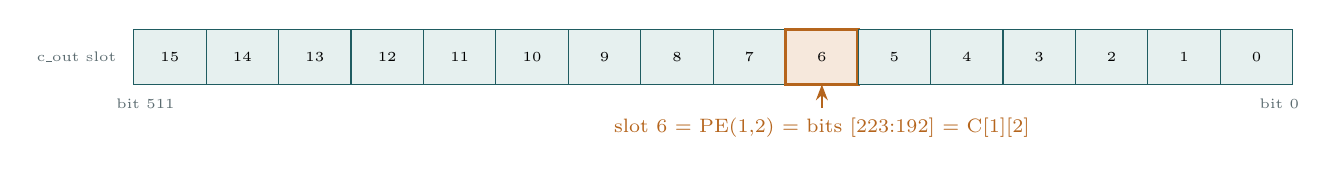
\begin{tikzpicture}[x=1mm,y=1mm]
    \foreach \s in {0,...,15} {
      \pgfmathtruncatemacro{\idx}{15-\s}
      \ifnum\idx=6
        \draw[copper, very thick, fill=coppert] (\s*9.2,0) rectangle ++(9.2,7);
      \else
        \draw[pcbmid, fill=tint] (\s*9.2,0) rectangle ++(9.2,7);
      \fi
      \node[font=\tiny] at (\s*9.2+4.6,3.5) {\idx};
    }
    \node[font=\tiny, text=muted, anchor=east] at (-1,3.5) {c\_out slot};
    \node[font=\tiny, text=muted] at (1.5,-2.5) {bit 511};
    \node[font=\tiny, text=muted] at (145.5,-2.5) {bit 0};
    \draw[wire] (87.4,-3) -- (87.4,0);
    \node[font=\scriptsize, text=copper, anchor=north] at (87.4,-3) {slot 6 = PE(1,2) = bits [223:192] = C[1][2]};
  \end{tikzpicture}}\\[1mm]
  \raggedright\small
  Two nested loops make 16 instances. The 16 accumulators are side by side in one 512-bit bus,
  \sig{c\_out}. \textbf{No logic}: it is just 512 wires, one group of 32 per PE.
\end{frame}

% =====================================================================
\section{Feeding the array}
\begin{frame}{12.\ RAM banks: why 4 + 4 small RAMs instead of one}
  \begin{columns}[T]
    \column{0.5\textwidth}
    \centering
    \resizebox{\linewidth}{!}{%
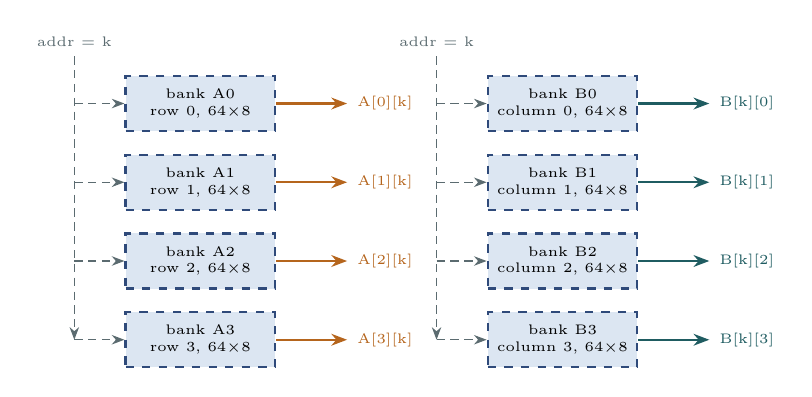
\begin{tikzpicture}[x=1mm,y=1mm]
      \foreach \n in {0,...,3} {
        \node[hard, minimum width=19mm, minimum height=7mm, font=\tiny] (a\n) at (16,-\n*10) {bank A\n\\row \n, 64$\times$8};
        \draw[wire] (a\n.east) -- ++(9,0) node[right,font=\tiny]{A[\n][k]};
        \node[hard, minimum width=19mm, minimum height=7mm, font=\tiny] (b\n) at (62,-\n*10) {bank B\n\\column \n, 64$\times$8};
        \draw[wireb] (b\n.east) -- ++(9,0) node[right,font=\tiny]{B[k][\n]};
      }
      \draw[ctl] (0,6) node[above,font=\tiny]{addr = k} -- (0,-30);
      \foreach \n in {0,...,3} \draw[ctl] (0,-\n*10) -- (a\n.west);
      \draw[ctl] (46,6) node[above,font=\tiny]{addr = k} -- (46,-30);
      \foreach \n in {0,...,3} \draw[ctl] (46,-\n*10) -- (b\n.west);
    \end{tikzpicture}}
    \column{0.48\textwidth}\small
    \begin{itemize}
      \item Every step the array needs \textbf{4 A values and 4 B values at once}. One RAM gives one byte per clock,
            so we use 8 RAMs, all read at the same address $k$.
      \item \textbf{Address map}: $A[i][k]$ at \hx{1000} + 64$i$ + $k$ (bank A$i$, address $k$);
            $B[k][j]$ at \hx{2000} + 4$k$ + $j$ (bank B$j$, address $k$).
      \item \textbf{M9K is synchronous}: the address is captured at a clock edge and the data comes out during the
            \textbf{next} cycle. That is the ``+1'' in $t = k + 1 + i + j$.
      \item Each bank uses 512 of the M9K's 9\,216 bits (5.6\,\%): 8 of 182 blocks.
    \end{itemize}
  \end{columns}
\end{frame}

% =====================================================================
\begin{frame}{13.\ The write path: one byte from the bus into its bank}
  \centering
  \resizebox{\textwidth}{!}{%
  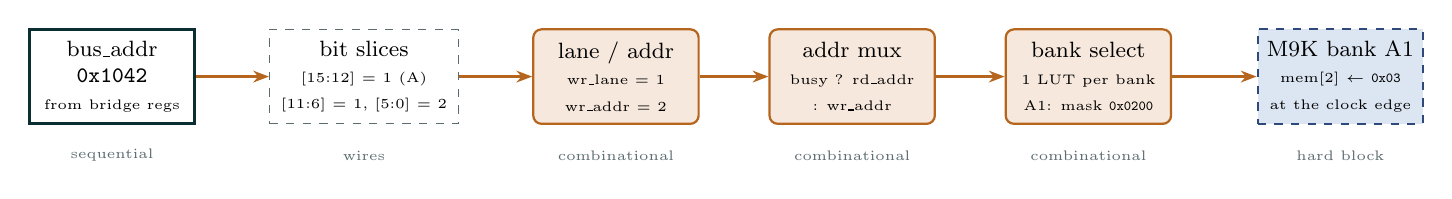
\begin{tikzpicture}[x=1mm,y=1mm]
    \node[seq, minimum width=21mm, minimum height=12mm] (ba) at (0,0) {bus\_addr\\\hx{1042}\\\tiny from bridge regs};
    \node[wires, minimum width=24mm, minimum height=12mm] (sl) at (32,0) {bit slices\\\tiny [15:12] = 1 (A)\\\tiny [11:6] = 1, [5:0] = 2};
    \node[comb, minimum width=21mm, minimum height=12mm] (mx) at (64,0) {lane / addr\\\tiny wr\_lane = 1\\\tiny wr\_addr = 2};
    \node[comb, minimum width=21mm, minimum height=12mm] (am) at (94,0) {addr mux\\\tiny busy ? rd\_addr\\\tiny : wr\_addr};
    \node[comb, minimum width=21mm, minimum height=12mm] (se) at (124,0) {bank select\\\tiny 1 LUT per bank\\\tiny A1: mask \hx{0200}};
    \node[hard, minimum width=21mm, minimum height=12mm] (rm) at (156,0) {M9K bank A1\\\tiny mem[2] $\leftarrow$ \hx{03}\\\tiny at the clock edge};
    \draw[wire] (ba) -- (sl); \draw[wire] (sl) -- (mx); \draw[wire] (mx) -- (am); \draw[wire] (am) -- (se); \draw[wire] (se) -- (rm);
    \foreach \x/\l in {0/sequential, 32/wires, 64/combinational, 94/combinational, 124/combinational, 156/hard block}
      \node[font=\tiny, text=muted] at (\x,-10) {\l};
  \end{tikzpicture}}

  \vspace{2mm}\raggedright\small
  \begin{itemize}
    \item The bank select is $\mathit{sel} = \sig{wr\_en} \wedge \neg\sig{wr\_sel} \wedge (\sig{wr\_lane} = n)$:
          exactly 4 inputs, so \textbf{one LUT per bank}. For bank A1 it is 1 only at input pattern 1001
          (address 9), so the mask is $2^9$ = \hx{0200}.
    \item \textbf{Why N and K\_MAX must be powers of 2:} ``row = offset / 64'' and ``k = offset mod 64'' become bit
          slices, which are free wires. Any other size would need divide logic. \sig{mm\_regs.sv} stops simulation
          with \sig{\$fatal} if they are not.
    \item The whole path is one clock: from the bridge's register to the M9K's write at the next edge.
  \end{itemize}
\end{frame}

% =====================================================================
\begin{frame}{14.\ The gate: why zeros are fed while the array fills and drains}
  \centering
  {\renewcommand{\cw}{1.32}
  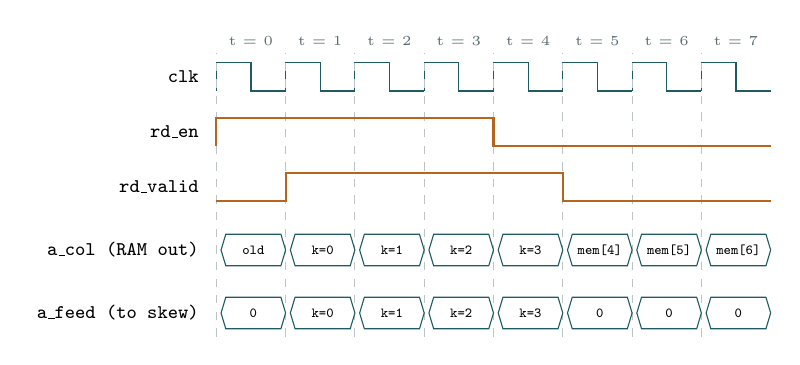
\begin{tikzpicture}[font=\scriptsize]
    \foreach \y/\s in {4.0/clk, 3.3/rd\_en, 2.6/rd\_valid, 1.8/a\_col (RAM out), 1.0/a\_feed (to skew)}
      \node[anchor=east, font=\scriptsize\ttfamily] at (-0.1,\y) {\s};
    \clockrow{4.0}{8}
    \foreach \c in {0,...,7} {\node[text=muted, font=\tiny] at ({(\c+0.5)*\cw},4.45) {t = \c};
                               \draw[muted!40, dashed] ({\c*\cw},0.7) -- ({\c*\cw},4.3);}
    \pulse{3.3}{0}{4}{8} \pulse{2.6}{1}{5}{8}
    \bus{0}{1}{1.8}{old} \bus{1}{2}{1.8}{k=0} \bus{2}{3}{1.8}{k=1} \bus{3}{4}{1.8}{k=2} \bus{4}{5}{1.8}{k=3}
    \bus{5}{6}{1.8}{mem[4]} \bus{6}{7}{1.8}{mem[5]} \bus{7}{8}{1.8}{mem[6]}
    \bus{0}{1}{1.0}{0} \bus{1}{2}{1.0}{k=0} \bus{2}{3}{1.0}{k=1} \bus{3}{4}{1.0}{k=2} \bus{4}{5}{1.0}{k=3}
    \bus{5}{6}{1.0}{0} \bus{6}{7}{1.0}{0} \bus{7}{8}{1.0}{0}
  \end{tikzpicture}}

  \vspace{2mm}\raggedright\small
  \begin{itemize}
    \item The RAM reads \textbf{every} cycle. In DRAIN the step counter keeps counting (4, 5, 6 \ldots), so the RAM
          shows \textbf{old data} from earlier jobs. Without the gate, the PEs would add garbage.
    \item \sig{rd\_valid} is \sig{rd\_en} delayed by \textbf{one flip-flop}, to line up with the RAM's one-clock delay.
    \item The gate is \sig{a\_feed = rd\_valid ? a\_col : 0}: 32 two-input AND functions per side (combinational).
  \end{itemize}
\end{frame}

% =====================================================================
\begin{frame}{15.\ The skew buffers for N = 4: lane $n$ waits $n$ clocks}
  \begin{columns}[T]
    \column{0.5\textwidth}
    \centering
    \resizebox{\linewidth}{!}{%
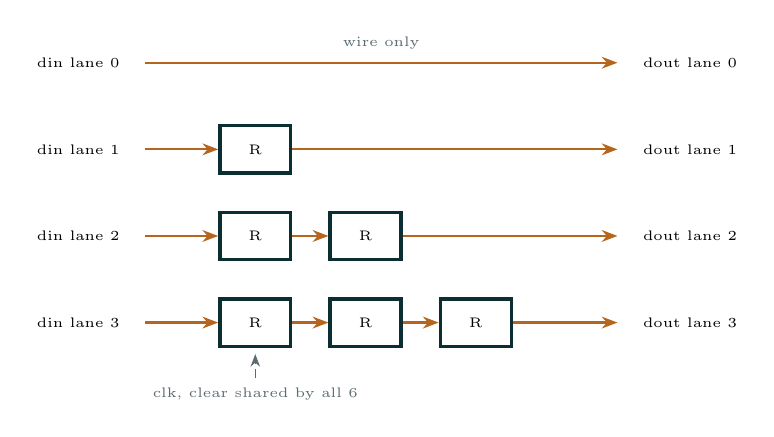
\begin{tikzpicture}[x=1mm,y=1mm]
      \foreach \n in {0,...,3} {
        \node[font=\tiny, anchor=east] at (-2,-\n*11) {din lane \n};
        \node[font=\tiny, anchor=west] at (62,-\n*11) {dout lane \n};
      }
      \draw[wire] (0,0) -- (60,0);
      \node[font=\tiny, text=muted, fill=white] at (30,2.5) {wire only};
      \foreach \n in {1,...,3} {
        \foreach \r in {1,...,\n} \node[seq, minimum width=9mm, minimum height=6mm, font=\tiny] (r\n\r) at (\r*14,-\n*11) {R};
        \draw[wire] (0,-\n*11) -- (r\n1.west);
        \ifnum\n>1
          \pgfmathtruncatemacro{\nm}{\n-1}
          \foreach \r in {1,...,\nm} {\pgfmathtruncatemacro{\rn}{\r+1} \draw[wire] (r\n\r) -- (r\n\rn);}
        \fi
        \draw[wire] (r\n\n.east) -- (60,-\n*11);
      }
      \draw[ctl] (14,-40) node[below,font=\tiny]{clk, clear shared by all 6} -- (14,-37);
    \end{tikzpicture}}
    \column{0.48\textwidth}\small
    \begin{itemize}
      \item Registers: $0 + 1 + 2 + 3 = 6$ per buffer, $\times$ 8 bits = \textbf{48 flip-flops}. Two buffers (A and B):
            \textbf{96}.
      \item A shift register maps to the LEs' \textbf{register chain}: flip-flop to flip-flop with no LUT and no
            general routing.
      \item No enable: the skew registers shift every clock and are zeroed by \sig{clear}.
      \item $A[i][k]$ leaves lane $i$ at step $k + 1 + i$. Example: $A[1][2]$ leaves lane 1 at step \textbf{4}.
      \item Lane 0 has no register, so PE(0,0)'s inputs come almost straight from the RAM (slide 31).
    \end{itemize}
  \end{columns}
\end{frame}

% =====================================================================
\section{Control}
\begin{frame}{16.\ The controller FSM (N = 4)}
  \centering
  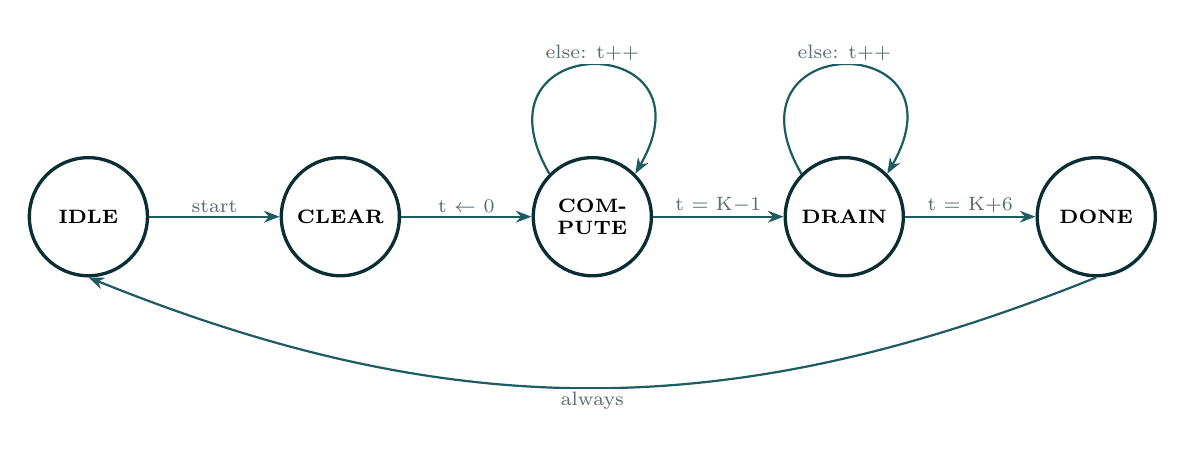
\begin{tikzpicture}[x=1mm,y=1mm, st/.style={circle, draw=pcb, very thick, fill=white, minimum size=15mm, font=\scriptsize\bfseries, align=center}]
    \node[st] (i) at (0,0) {IDLE};
    \node[st] (c) at (32,0) {CLEAR};
    \node[st] (p) at (64,0) {COM-\\PUTE};
    \node[st] (d) at (96,0) {DRAIN};
    \node[st] (o) at (128,0) {DONE};
    \draw[wireb] (i) -- node[w,above]{start} (c);
    \draw[wireb] (c) -- node[w,above]{t $\leftarrow$ 0} (p);
    \draw[wireb] (p) -- node[w,above]{t = K$-$1} (d);
    \draw[wireb] (d) -- node[w,above]{t = K+6} (o);
    \draw[wireb] (o.south) to[bend left=22] node[w,below]{always} (i.south);
    \draw[wireb] (p.north west) to[out=120,in=60,looseness=5] node[w,above]{else: t++} (p.north east);
    \draw[wireb] (d.north west) to[out=120,in=60,looseness=5] node[w,above]{else: t++} (d.north east);
  \end{tikzpicture}

  \vspace{1mm}\small
  \begin{tabular}{@{}lccccc l@{}}
    \toprule
    \textbf{State} & \sig{busy} & \sig{clear} & \sig{rd\_en} & \sig{array\_en} & \sig{done} & \textbf{Cycles} \\
    \midrule
    IDLE    & 0 & 0 & 0 & 0 & 0 & until \sig{start} \\
    CLEAR   & 1 & 1 & 0 & 0 & 0 & 1 \\
    COMPUTE & 1 & 0 & 1 & 1 & 0 & K (t = 0 \ldots K$-$1) \\
    DRAIN   & 1 & 0 & 0 & 1 & 0 & 2N$-$1 = 7 (t = K \ldots K+6) \\
    DONE    & 1 & 0 & 0 & 0 & 1 & 1 \\
    \bottomrule
  \end{tabular}\\[1mm]
  \raggedright\footnotesize
  A \textbf{Moore} machine: every output depends on the state only. The same step counter \sig{t} is the RAM read
  address in COMPUTE.
\end{frame}

% =====================================================================
\begin{frame}{17.\ The FSM as hardware}
  \centering
  \resizebox{0.95\textwidth}{!}{%
  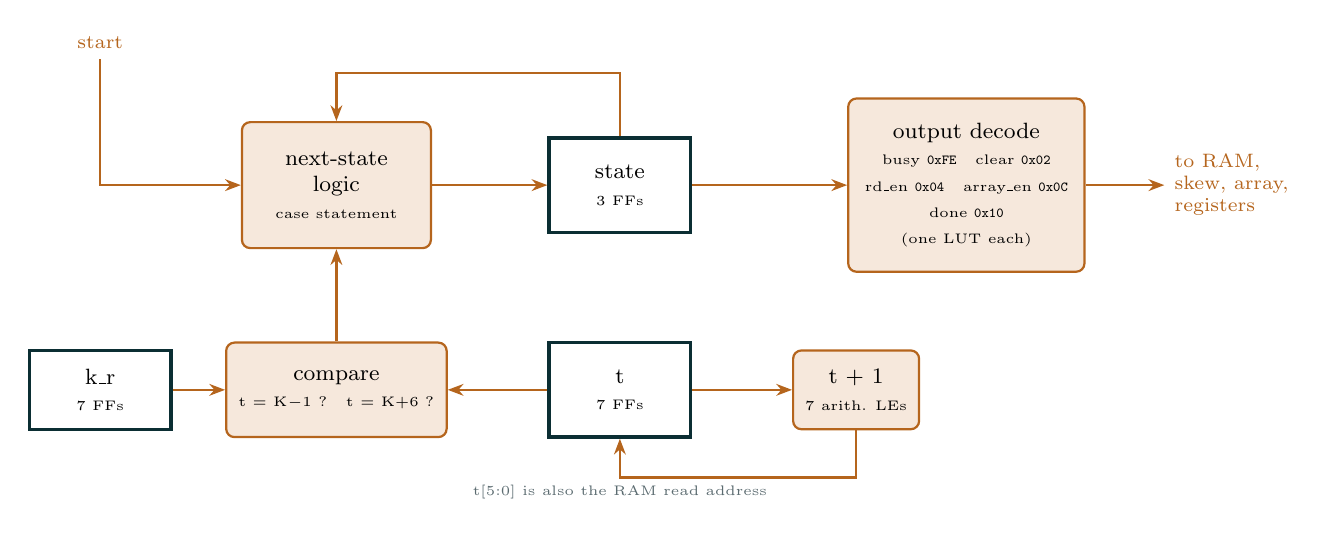
\begin{tikzpicture}[x=1mm,y=1mm]
    \node[comb, minimum width=24mm, minimum height=16mm] (ns) at (30,20) {next-state\\logic\\\tiny case statement};
    \node[seq,  minimum width=18mm, minimum height=12mm] (st) at (66,20) {state\\\tiny 3 FFs};
    \node[comb, minimum width=30mm, minimum height=22mm] (od) at (110,20) {output decode\\\tiny busy \hx{FE}\quad clear \hx{02}\\\tiny rd\_en \hx{04}\quad array\_en \hx{0C}\\\tiny done \hx{10}\\\tiny (one LUT each)};
    \node[seq,  minimum width=18mm, minimum height=12mm] (t) at (66,-6) {t\\\tiny 7 FFs};
    \node[comb, minimum width=16mm, minimum height=10mm] (inc) at (96,-6) {t + 1\\\tiny 7 arith. LEs};
    \node[comb, minimum width=28mm, minimum height=12mm] (cmp) at (30,-6) {compare\\\tiny t = K$-$1 ?\quad t = K+6 ?};
    \node[seq,  minimum width=18mm, minimum height=10mm] (k) at (0,-6) {k\_r\\\tiny 7 FFs};
    \draw[wire] (ns) -- (st);
    \draw[wire] (st) -- (od);
    \draw[wire] (od.east) -- ++(10,0) node[right,font=\scriptsize,align=left]{to RAM,\\skew, array,\\registers};
    \draw[wire] (st.north) -- ++(0,8) -| (ns.north);
    \draw[wire] (t) -- (inc);
    \draw[wire] (inc.south) -- ++(0,-6) -| (t.south);
    \draw[wire] (t.west) -- (cmp.east);
    \draw[wire] (k) -- (cmp);
    \draw[wire] (cmp.north) -- (ns.south);
    \draw[wire] (0,36) node[above,font=\scriptsize]{start} -- (0,20) -- (ns.west);
    \node[font=\tiny, text=muted] at (66,-19) {t[5:0] is also the RAM read address};
  \end{tikzpicture}}

  \vspace{1mm}\raggedright\small
  \begin{itemize}
    \item \textbf{Sequential}: \sig{state} (3), \sig{t} (7), \sig{k\_r} (7) = \textbf{17 flip-flops}.
    \item \textbf{Combinational}: next-state logic, the $+1$ for \sig{t} (carry chain), two 7-bit equality
          compares, output decode. With IDLE=0 \ldots DONE=4, \sig{array\_en} is true for states 2 and 3, so its mask is
          \hx{0C}.
    \item Quartus may re-encode the state as one-hot; then each output is about one flip-flop.
  \end{itemize}
\end{frame}

% =====================================================================
\section{Time}
\begin{frame}{18.\ One 4$\times$4 job (K = 4), clock by clock}
  \centering
  \resizebox{0.94\textwidth}{!}{%
  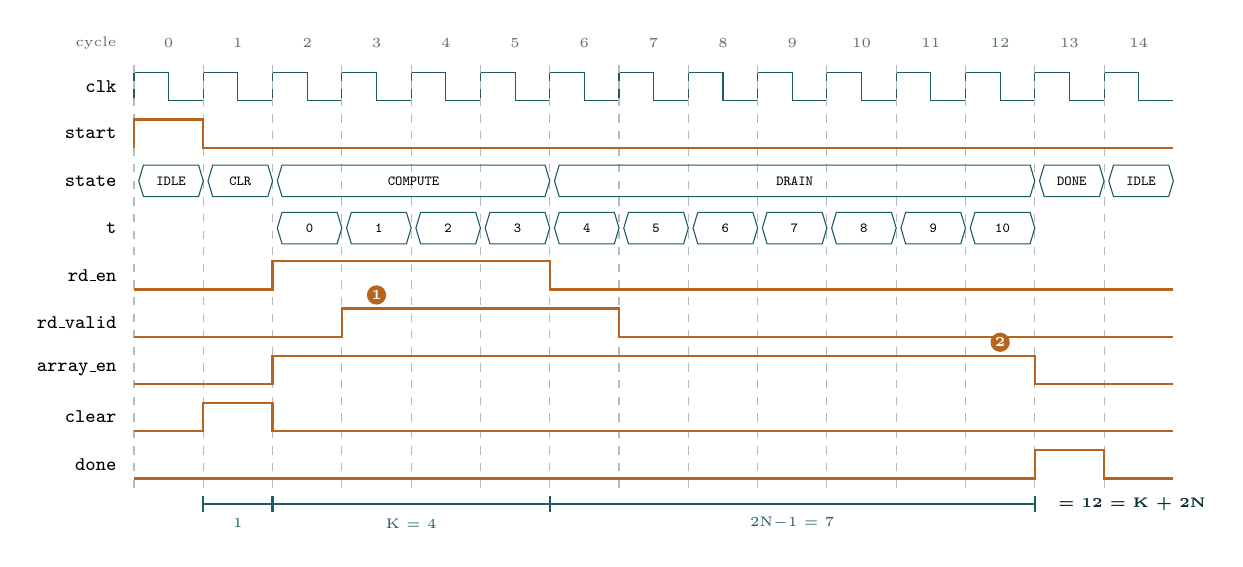
\begin{tikzpicture}[font=\scriptsize]
    \foreach \y/\s in {5.6/clk, 5.0/start, 4.4/state, 3.8/t, 3.2/rd\_en, 2.6/rd\_valid, 2.0/array\_en, 1.4/clear, 0.8/done}
      \node[anchor=east, font=\scriptsize\ttfamily] at (-0.1,\y) {\s};
    \clockrow{5.6}{15}
    \foreach \c in {0,...,14} {
      \draw[muted!45, dashed] (\c*\cw,0.5) -- (\c*\cw,5.95);
      \node[text=muted, font=\tiny] at (\c*\cw+\cw/2,6.15) {\c};
    }
    \node[text=muted, font=\tiny, anchor=east] at (-0.1,6.15) {cycle};
    \pulse{5.0}{0}{1}{15}
    \bus{0}{1}{4.4}{IDLE} \bus{1}{2}{4.4}{CLR} \bus{2}{6}{4.4}{COMPUTE} \bus{6}{13}{4.4}{DRAIN}
    \bus{13}{14}{4.4}{DONE} \bus{14}{15}{4.4}{IDLE}
    \foreach \c in {2,...,12} { \pgfmathtruncatemacro{\tv}{\c-2} \bus{\c}{\c+1}{3.8}{\tv} }
    \pulse{3.2}{2}{6}{15}
    \pulse{2.6}{3}{7}{15}
    \pulse{2.0}{2}{13}{15}
    \pulse{1.4}{1}{2}{15}
    \pulse{0.8}{13}{14}{15}
    \node[stn] at (3.5*\cw,2.95) {1};
    \node[stn] at (12.5*\cw,2.35) {2};
    \draw[pcbmid, thick] (1*\cw,0.3) -- (13*\cw,0.3);
    \foreach \x in {1,2,6,13} \draw[pcbmid, thick] (\x*\cw,0.2) -- (\x*\cw,0.4);
    \node[font=\tiny, text=pcbmid] at (1.5*\cw,0.05) {1};
    \node[font=\tiny, text=pcbmid] at (4*\cw,0.05) {K = 4};
    \node[font=\tiny, text=pcbmid] at (9.5*\cw,0.05) {2N$-$1 = 7};
    \node[font=\tiny\bfseries, text=pcb, anchor=west] at (13.2*\cw,0.3) {= 12 = K + 2N};
  \end{tikzpicture}}

  \vspace{0mm}\raggedright\scriptsize
  \textcolor{copper}{\textbf{1}} cycle 3 (t = 1): \sig{rd\_valid} = 1, so A[$\cdot$][0] and B[0][$\cdot$] reach PE(0,0).
  \sig{rd\_valid} is \sig{rd\_en} one register later, because the M9K returns data one clock after the address:
  that is the ``+1'' in $t = k+1+i+j$.\quad
  \textcolor{copper}{\textbf{2}} cycle 12 (t = 10): the last MAC, PE(3,3) with k = 3. \sig{done} follows, and C is ready.
\end{frame}

% =====================================================================
\begin{frame}{19.\ The wavefront: which PE works at each step (K = 4)}
  \centering
  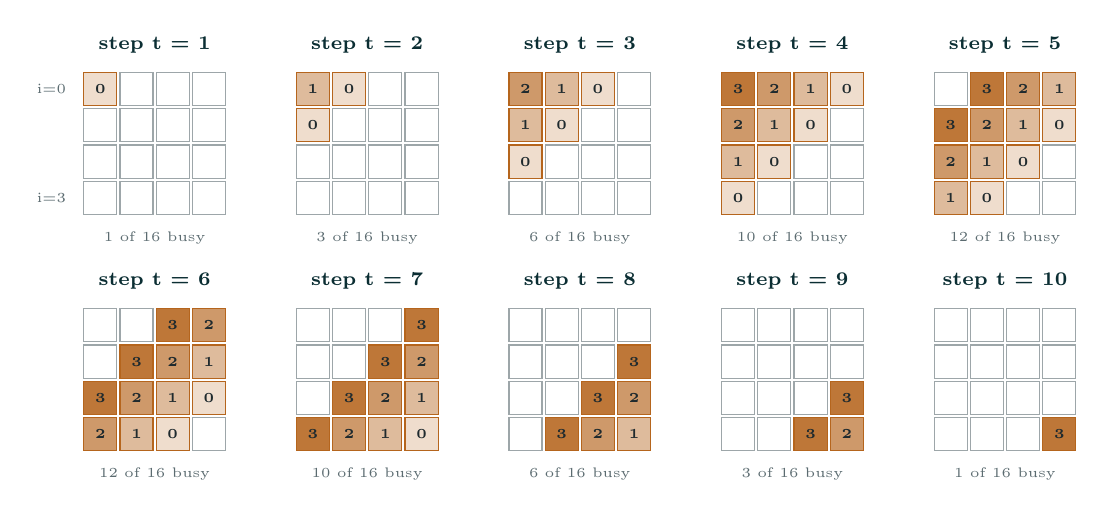
\begin{tikzpicture}[x=1mm,y=1mm]
    \foreach \t in {1,...,10} {
      \pgfmathtruncatemacro{\col}{mod(\t-1,5)}
      \pgfmathtruncatemacro{\row}{(\t-1)/5}
      \pgfmathsetmacro{\ox}{\col*27}
      \pgfmathsetmacro{\oy}{-\row*30}
      \foreach \i in {0,...,3} \foreach \j in {0,...,3} {
        \pgfmathtruncatemacro{\k}{\t-1-\i-\j}
        \ifnum\k<0
          \draw[muted!60, fill=white] (\ox+\j*4.6,\oy-\i*4.6) rectangle ++(4.2,-4.2);
        \else\ifnum\k>3
          \draw[muted!60, fill=white] (\ox+\j*4.6,\oy-\i*4.6) rectangle ++(4.2,-4.2);
        \else
          \pgfmathtruncatemacro{\shade}{22+22*\k}
          \draw[copper, fill=copper!\shade] (\ox+\j*4.6,\oy-\i*4.6) rectangle ++(4.2,-4.2);
          \node[font=\tiny\bfseries, text=ink] at (\ox+\j*4.6+2.1,\oy-\i*4.6-2.1) {\k};
        \fi\fi
      }
      \node[font=\scriptsize\bfseries, text=pcb] at (\ox+9,\oy+3.5) {step t = \t};
    }
    \foreach \t/\n in {1/1,2/3,3/6,4/10,5/12,6/12,7/10,8/6,9/3,10/1} {
      \pgfmathtruncatemacro{\col}{mod(\t-1,5)}
      \pgfmathtruncatemacro{\row}{(\t-1)/5}
      \node[font=\tiny, text=muted] at (\col*27+9,-\row*30-21) {\n\ of 16 busy};
    }
    \node[font=\tiny, text=muted, anchor=east] at (-1,-2.1) {i=0};
    \node[font=\tiny, text=muted, anchor=east] at (-1,-15.9) {i=3};
  \end{tikzpicture}

  \vspace{1mm}\raggedright\footnotesize
  \begin{itemize}
    \item The number in a cell is \textbf{k}: PE(i,j) multiplies $A[i][k]\cdot B[k][j]$ at step
          $\mathbf{t = k + 1 + i + j}$ (the +1 is the RAM read latency).
    \item Total work: $1+3+6+10+12+12+10+6+3+1 = \mathbf{64} = N^2K$ MACs in 11 steps.
          Never all 16 busy, so utilization is $64/(16\times11) = $ \textbf{36\%}. With K = 64 it is \textbf{90.1\%}.
  \end{itemize}
\end{frame}

% =====================================================================
\begin{frame}{20.\ Why DRAIN is 2N $-$ 1 = 7, and the total is K + 2N}
  \begin{columns}[T]
    \column{0.52\textwidth}\small
    Follow the \textbf{last} value, $A[3][K{-}1]$:
    \begin{enumerate}
      \item read from RAM at the last COMPUTE step: \textbf{t = K$-$1}
      \item out of the M9K one clock later: \textbf{+1}
      \item through skew lane 3 (3 registers): \textbf{+3}
      \item through PE(3,0), PE(3,1), PE(3,2) to PE(3,3): \textbf{+3}
    \end{enumerate}
    Last MAC at $t = K - 1 + 1 + 3 + 3 = K + 6 = K + 2N - 2$.\\[1mm]
    DRAIN covers $t = K \ldots K+6$: \textbf{7 = 2N $-$ 1 cycles}.\\[1mm]
    Total busy: 1 (CLEAR) + K (COMPUTE) + 7 (DRAIN) = \textbf{K + 2N}.
    \column{0.45\textwidth}\small
    \resizebox{\linewidth}{!}{%
\begin{tabular}{@{}lrr@{}}
      \toprule
       & \textbf{K = 4} & \textbf{K = 64} \\
      \midrule
      CLEAR & 1 & 1 \\
      COMPUTE & 4 & 64 \\
      DRAIN & 7 & 7 \\
      \textbf{Total (PERF\_TOTAL)} & \textbf{12} & \textbf{72} \\
      Array enabled (PERF\_COMPUTE) & 11 & 71 \\
      Utilization & 36.4\,\% & 90.1\,\% \\
      \bottomrule
    \end{tabular}}\\[2mm]
    The overhead (CLEAR + DRAIN = 8 cycles) is \textbf{fixed}. That is why a large K is efficient and a small K is not.
  \end{columns}
\end{frame}

% =====================================================================
\section{Results}
\begin{frame}{21.\ Reading C: a 16-to-1 multiplexer, then one register}
  \centering
  \resizebox{0.95\textwidth}{!}{%
  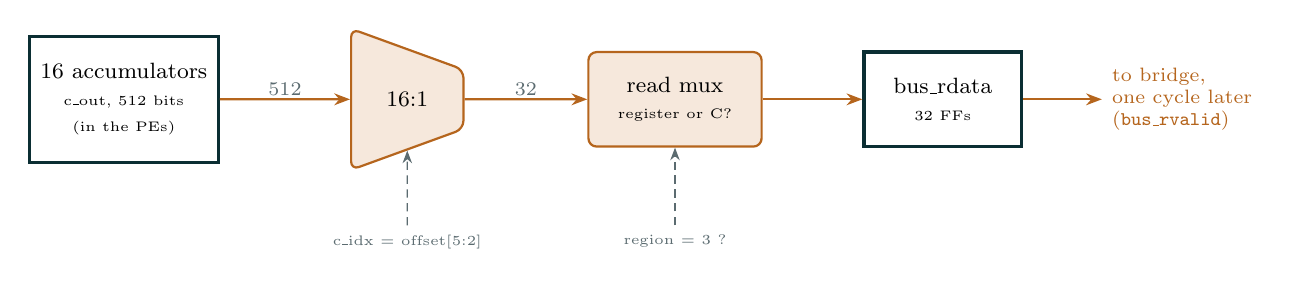
\begin{tikzpicture}[x=1mm,y=1mm]
    \node[seq, minimum width=24mm, minimum height=16mm] (acc) at (0,0) {16 accumulators\\\tiny c\_out, 512 bits\\\tiny (in the PEs)};
    \node[comb, trapezium, trapezium angle=70, shape border rotate=270, minimum width=18mm, minimum height=14mm] (mx) at (36,0) {16:1};
    \node[comb, minimum width=22mm, minimum height=12mm] (rm) at (70,0) {read mux\\\tiny register or C?};
    \node[seq, minimum width=20mm, minimum height=12mm] (rd) at (104,0) {bus\_rdata\\\tiny 32 FFs};
    \draw[wire] (acc) -- node[w,above]{512} (mx);
    \draw[wire] (mx) -- node[w,above]{32} (rm);
    \draw[wire] (rm) -- (rd);
    \draw[wire] (rd.east) -- ++(10,0) node[right,font=\scriptsize,align=left]{to bridge,\\one cycle later\\(\sig{bus\_rvalid})};
    \draw[ctl] (36,-16) node[below,font=\tiny]{c\_idx = offset[5:2]} -- (mx.south);
    \draw[ctl] (70,-16) node[below,font=\tiny]{region = 3 ?} -- (rm.south);
  \end{tikzpicture}}

  \vspace{2mm}\raggedright\small
  \begin{itemize}
    \item Reading \hx{3018}: offset \hx{018} = 24, so \sig{c\_idx} = 24 / 4 = \textbf{6} = PE(1,2) (bit slicing again: free).
    \item A 4:1 multiplexer needs 2 LUTs, so 16:1 needs 10 LUTs \textbf{per bit}: about \textbf{320 LUTs} for 32 bits.
          For 8$\times$8 it grows to about 1\,344, a hidden cost of output-stationary arrays.
    \item The answer is registered in \sig{bus\_rdata} and flagged by \sig{bus\_rvalid} exactly one cycle after the read
          is accepted (checked by SVA and the formal proof).
  \end{itemize}
\end{frame}

% =====================================================================
\begin{frame}{22.\ Registers and performance counters}
  \begin{columns}[T]
    \column{0.5\textwidth}\small
    \textbf{Register map} (\sig{mm\_regs.sv})\\[1mm]
    {\footnotesize
    \begin{tabular}{@{}ll@{}}
      \hx{0000} CTRL & bit 0 START, bit 1 SOFT\_RESET \\
      \hx{0004} STATUS & bit 0 BUSY, bit 1 DONE (sticky) \\
      \hx{0008} CFG\_K & K, 1 \ldots 64 \\
      \hx{000C} INFO & N, K\_MAX, version \\
      \hx{0010}--\hx{0020} & 5 performance counters \\
      \hx{1000} A\_BUF & A[i][k] at + 64$i$ + $k$ \\
      \hx{2000} B\_BUF & B[k][j] at + 4$k$ + $j$ \\
      \hx{3000} C\_BUF & C[i][j] at + 4(4$i$ + $j$) \\
    \end{tabular}}
    \column{0.47\textwidth}\small
    \textbf{Counters after our K = 4 job}\\[1mm]
    {\footnotesize
    \begin{tabular}{@{}lrl@{}}
      \toprule
      PERF\_TOTAL & 12 & START $\rightarrow$ DONE \\
      PERF\_COMPUTE & 11 & array enabled \\
      PERF\_FILLDRAIN & 11 & enabled, some PE idle \\
      PERF\_MACS & 64 & +16 per read step \\
      \bottomrule
    \end{tabular}}\\[2mm]
    Each counter = \textbf{32 flip-flops} (sequential) + a 32-bit adder in arithmetic-mode LEs
    (combinational). PERF\_FILLDRAIN = 11 because with K = 4 no step has all 16 PEs busy.
  \end{columns}
\end{frame}

% =====================================================================
\section{End to end}
\begin{frame}{23.\ End to end: one example, followed all the way}
  \centering
  \[
  A=\begin{pmatrix} 1&2&0&1\\ \textcolor{copper}{2}&\textcolor{copper}{-1}&\colorbox{coppert}{\textbf{3}}&\textcolor{copper}{1}\\ 0&1&1&2\\ 1&0&-2&1 \end{pmatrix}
  \quad
  B=\begin{pmatrix} 1&0&\textcolor{pcbmid}{2}&1\\ 0&1&\textcolor{pcbmid}{1}&-1\\ 2&1&\textcolor{pcbmid}{\mathbf{2}}&1\\ 1&2&\textcolor{pcbmid}{1}&0 \end{pmatrix}
  \quad
  C=A\cdot B=\begin{pmatrix} 2&4&5&-1\\ 9&4&\colorbox{coppert}{\textbf{10}}&6\\ 4&6&5&0\\ -2&0&-1&-1 \end{pmatrix}
  \]
  \raggedright\small
  \begin{itemize}
    \item We follow \textbf{A[1][2] = 3} into the chip (byte \hx{03}, address \hx{1042}), through the array,
          and \textbf{C[1][2] = 10} back out (address \hx{3018}).
    \item $C[1][2] = 2\cdot2 + (-1)\cdot1 + 3\cdot2 + 1\cdot1 = 4 - 1 + 6 + 1 = \mathbf{10}$, built inside PE(1,2).
    \item Three stages: \textbf{in} (PC $\rightarrow$ RAM), \textbf{compute} (RAM $\rightarrow$ PEs), \textbf{out}
          (PE $\rightarrow$ PC). Every step is marked combinational or sequential.
  \end{itemize}
\end{frame}

% =====================================================================
\begin{frame}{24.\ The whole journey on one page}
  \centering
  \resizebox{\textwidth}{!}{%
  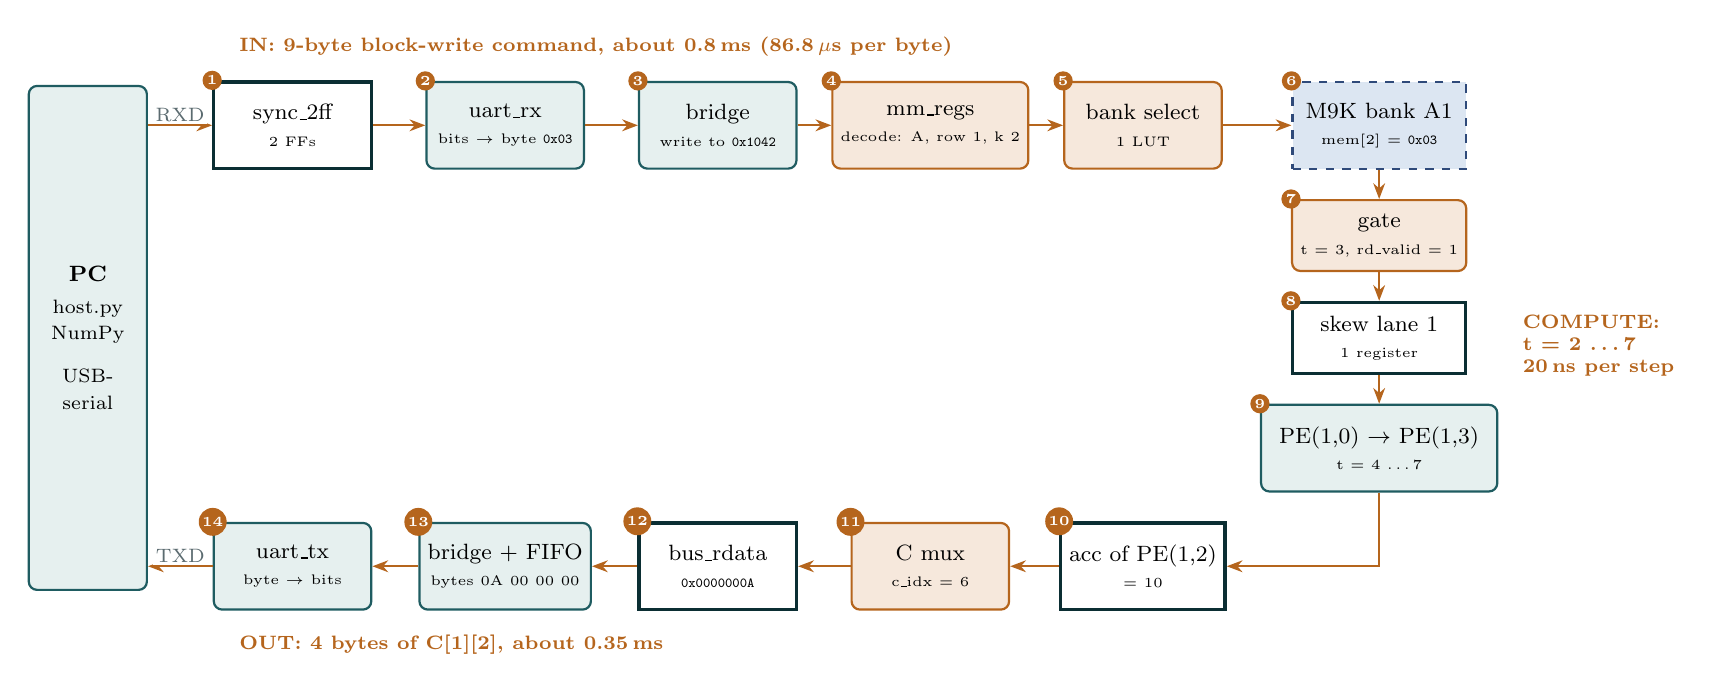
\begin{tikzpicture}[x=1mm,y=1mm]
    \node[blk, minimum width=15mm, minimum height=64mm] (pc) at (-24,9) {\textbf{PC}\\[2pt]\scriptsize host.py\\\scriptsize NumPy\\[6pt]\scriptsize USB-\\\scriptsize serial};
    % in
    \node[seq,  minimum width=20mm, minimum height=11mm] (s1) at (2,36)  {sync\_2ff\\\tiny 2 FFs};
    \node[mix,  minimum width=20mm, minimum height=11mm] (s2) at (29,36) {uart\_rx\\\tiny bits $\rightarrow$ byte \hx{03}};
    \node[mix,  minimum width=20mm, minimum height=11mm] (s3) at (56,36) {bridge\\\tiny write to \hx{1042}};
    \node[comb, minimum width=20mm, minimum height=11mm] (s4) at (83,36) {mm\_regs\\\tiny decode: A, row 1, k 2};
    \node[comb, minimum width=20mm, minimum height=11mm] (s5) at (110,36) {bank select\\\tiny 1 LUT};
    \node[hard, minimum width=22mm, minimum height=11mm] (s6) at (140,36) {M9K bank A1\\\tiny mem[2] = \hx{03}};
    % compute
    \node[comb, minimum width=22mm, minimum height=9mm] (s7) at (140,22) {gate\\\tiny t = 3, rd\_valid = 1};
    \node[seq,  minimum width=22mm, minimum height=9mm] (s8) at (140,9) {skew lane 1\\\tiny 1 register};
    \node[mix,  minimum width=30mm, minimum height=11mm] (s9) at (140,-5) {PE(1,0) $\rightarrow$ PE(1,3)\\\tiny t = 4 \ldots 7};
    % out
    \node[seq,  minimum width=20mm, minimum height=11mm] (s10) at (110,-20) {acc of PE(1,2)\\\tiny = 10};
    \node[comb, minimum width=20mm, minimum height=11mm] (s11) at (83,-20) {C mux\\\tiny c\_idx = 6};
    \node[seq,  minimum width=20mm, minimum height=11mm] (s12) at (56,-20) {bus\_rdata\\\tiny \hx{0000000A}};
    \node[mix,  minimum width=20mm, minimum height=11mm] (s13) at (29,-20) {bridge + FIFO\\\tiny bytes 0A 00 00 00};
    \node[mix,  minimum width=20mm, minimum height=11mm] (s14) at (2,-20) {uart\_tx\\\tiny byte $\rightarrow$ bits};
    \draw[wire] (pc.east |- s1) -- node[w,above]{RXD} (s1);
    \foreach \a/\b in {s1/s2, s2/s3, s3/s4, s4/s5, s5/s6} \draw[wire] (\a) -- (\b);
    \draw[wire] (s6) -- (s7); \draw[wire] (s7) -- (s8); \draw[wire] (s8) -- (s9);
    \draw[wire] (s9.south) |- (s10.east);
    \foreach \a/\b in {s10/s11, s11/s12, s12/s13, s13/s14} \draw[wire] (\a) -- (\b);
    \draw[wire] (s14) -- node[w,above]{TXD} (pc.east |- s14);
    \foreach \s/\n in {s1/1, s2/2, s3/3, s4/4, s5/5, s6/6, s7/7, s8/8, s9/9, s10/10, s11/11, s12/12, s13/13, s14/14}
      \node[stn] at (\s.north west) {\n};
    \node[font=\scriptsize\bfseries, text=copper, anchor=west] at (-6,46) {IN: 9-byte block-write command, about 0.8\,ms (86.8\,$\mu$s per byte)};
    \node[font=\scriptsize\bfseries, text=copper, anchor=west, align=left] at (157,8) {COMPUTE:\\t = 2 \ldots 7\\20\,ns per step};
    \node[font=\scriptsize\bfseries, text=copper, anchor=west] at (-6,-30) {OUT: 4 bytes of C[1][2], about 0.35\,ms};
  \end{tikzpicture}}

  \vspace{1mm}\raggedright\footnotesize
  14 stations. White = flip-flops, copper = logic, dashed blue = hard block, teal = both. The next four slides zoom in.
\end{frame}

% =====================================================================
\begin{frame}{25.\ Stage 1 --- IN: from the PC into RAM bank A1 (stations 1--6)}
  \centering
  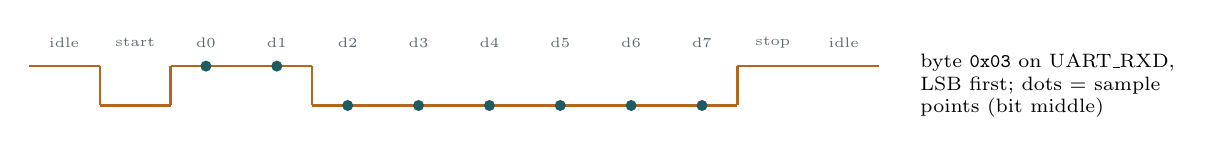
\begin{tikzpicture}[x=1mm,y=1mm]
    \uart{0}{1,0,1,1,0,0,0,0,0,0,1,1}
    \foreach \n/\s in {0/idle, 1/start, 2/d0, 3/d1, 4/d2, 5/d3, 6/d4, 7/d5, 8/d6, 9/d7, 10/stop, 11/idle}
      \node[font=\tiny, text=muted] at (\n*9+4.5,8) {\s};
    \foreach \n in {2,...,9} \fill[pcbmid] (\n*9+4.5,{(\n<4)*5}) circle (0.7);
    \node[font=\scriptsize, anchor=west, align=left] at (112,2.5) {byte \hx{03} on UART\_RXD,\\LSB first; dots = sample\\points (bit middle)};
  \end{tikzpicture}\\[2mm]
  \resizebox{\textwidth}{!}{%
  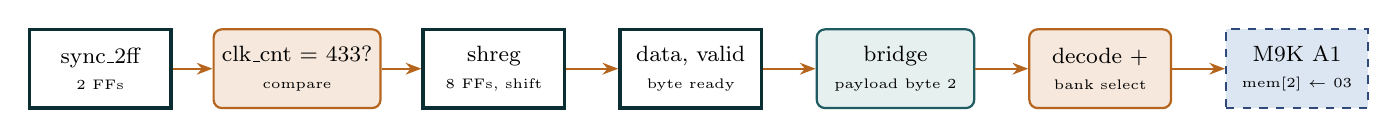
\begin{tikzpicture}[x=1mm,y=1mm]
    \node[seq,  minimum width=18mm, minimum height=10mm] (a) at (0,0)   {sync\_2ff\\\tiny 2 FFs};
    \node[comb, minimum width=18mm, minimum height=10mm] (b) at (25,0)  {clk\_cnt = 433?\\\tiny compare};
    \node[seq,  minimum width=18mm, minimum height=10mm] (c) at (50,0)  {shreg\\\tiny 8 FFs, shift};
    \node[seq,  minimum width=18mm, minimum height=10mm] (d) at (75,0)  {data, valid\\\tiny byte ready};
    \node[mix,  minimum width=20mm, minimum height=10mm] (e) at (101,0) {bridge\\\tiny payload byte 2};
    \node[comb, minimum width=18mm, minimum height=10mm] (f) at (127,0) {decode +\\\tiny bank select};
    \node[hard, minimum width=18mm, minimum height=10mm] (g) at (152,0) {M9K A1\\\tiny mem[2] $\leftarrow$ 03};
    \foreach \x/\y in {a/b, b/c, c/d, d/e, e/f, f/g} \draw[wire] (\x) -- (\y);
  \end{tikzpicture}}

  \vspace{1mm}\raggedright\footnotesize
  \begin{itemize}
    \item At 115\,200 baud one bit is 434 clocks (8.68\,$\mu$s). \sig{uart\_rx} counts to the middle of each bit
          (counter + compare) and shifts the bit into \sig{shreg}: d0 = 1, d1 = 1, the rest 0, so \hx{03}.
    \item The host sent \sig{42 40 10 04 00 02 FF 03 01}: \sig{'B'}, address \hx{1040}, length 4, then row 1 of A.
          Our \hx{03} is payload byte 2, so the bridge writes it to \hx{1040} + 2 = \hx{1042}.
    \item Decode (slide 13): bank A1, address 2. The M9K stores it at the next clock edge.
  \end{itemize}
\end{frame}

% =====================================================================
\begin{frame}{26.\ Stage 2 --- COMPUTE: one RAM read, four PEs}
  \centering
  \resizebox{\textwidth}{!}{%
  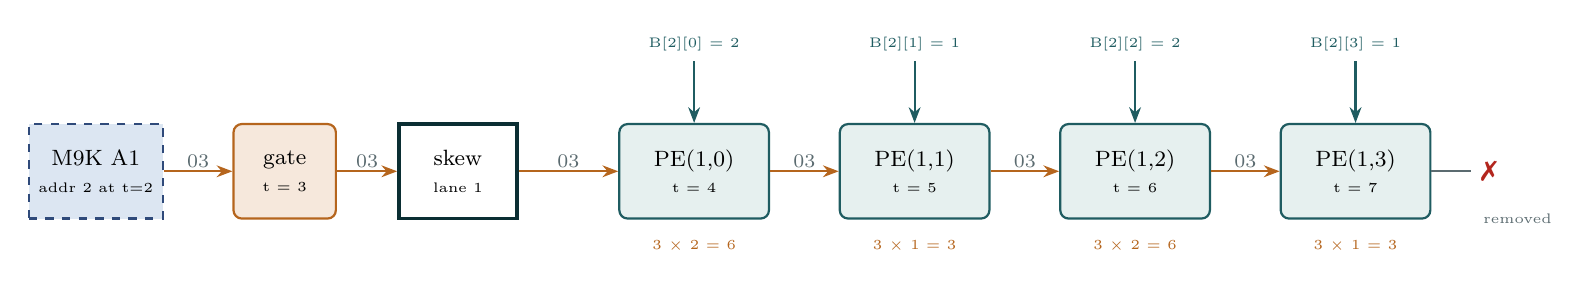
\begin{tikzpicture}[x=1mm,y=1mm]
    \node[hard, minimum width=17mm, minimum height=12mm] (r) at (0,0)   {M9K A1\\\tiny addr 2 at t=2};
    \node[comb, minimum width=13mm, minimum height=12mm] (g) at (24,0)  {gate\\\tiny t = 3};
    \node[seq,  minimum width=15mm, minimum height=12mm] (s) at (46,0)  {skew\\\tiny lane 1};
    \foreach \j/\st/\bv/\pv in {0/4/2/6, 1/5/1/3, 2/6/2/6, 3/7/1/3} {
      \node[mix, minimum width=19mm, minimum height=12mm] (p\j) at (76+\j*28,0) {PE(1,\j)\\\tiny t = \st};
      \draw[wireb] (76+\j*28,14) node[above,font=\tiny]{B[2][\j] = \bv} -- (p\j.north);
      \node[font=\tiny, text=copper, anchor=north] at (76+\j*28,-7.5) {3 $\times$ \bv\ = \pv};
    }
    \draw[wire] (r) -- node[w,above]{03} (g); \draw[wire] (g) -- node[w,above]{03} (s);
    \draw[wire] (s) -- node[w,above]{03} (p0);
    \foreach \a/\b in {0/1, 1/2, 2/3} \draw[wire] (p\a) -- node[w,above]{03} (p\b);
    \draw[muted, thick] (p3.east) -- ++(5,0) node[right, text=bad]{\ding{55}};
    \node[font=\tiny, text=muted, anchor=west] at (175,-6) {removed};
  \end{tikzpicture}}

  \vspace{2mm}\raggedright\small
  \resizebox{\textwidth}{!}{%
\begin{tabular}{@{}lll@{}}
    \toprule
    \textbf{Step} & \textbf{What happens to the value 3} & \textbf{Kind} \\
    \midrule
    t = 2 & address 2 is captured by the M9K at the clock edge & hard (sequential) \\
    t = 3 & RAM outputs \hx{03}; \sig{rd\_valid} = 1, so the gate passes it; the skew register takes it at the edge & comb $\rightarrow$ seq \\
    t = 4 \ldots 7 & each PE multiplies it by its B value and adds; \sig{a\_out} passes it right at every edge & comb + seq \\
    after t = 7 & PE(1,3)'s \sig{a\_out} drives nothing, so the value is simply dropped & --- \\
    \bottomrule
  \end{tabular}}\\[1mm]
  \footnotesize One RAM read feeds \textbf{four} multiplies: this reuse is the point of a systolic array.
\end{frame}

% =====================================================================
\begin{frame}{27.\ Inside PE(1,2): combinational vs sequential in time}
  \centering
  {\renewcommand{\cw}{1.75}
  \resizebox{0.95\textwidth}{!}{%
  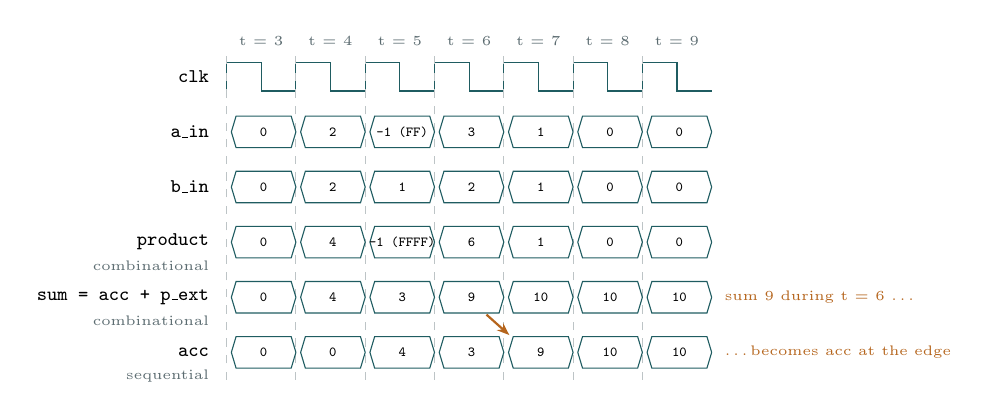
\begin{tikzpicture}[font=\scriptsize]
    \foreach \y/\s/\k in {4.4/clk/, 3.7/a\_in/, 3.0/b\_in/, 2.3/product/comb, 1.6/sum = acc + p\_ext/comb, 0.9/acc/seq}
      \node[anchor=east, font=\scriptsize\ttfamily] at (-0.1,\y) {\s};
    \foreach \y/\k in {2.3/combinational, 1.6/combinational, 0.9/sequential}
      \node[anchor=east, font=\tiny, text=muted] at (-0.1,\y-0.3) {\k};
    \clockrow{4.4}{7}
    \foreach \c in {0,...,6} {
      \pgfmathtruncatemacro{\tv}{\c+3}
      \node[text=muted, font=\tiny] at ({(\c+0.5)*\cw},4.85) {t = \tv};
      \draw[muted!40, dashed] ({\c*\cw},0.55) -- ({\c*\cw},4.7);
    }
    \foreach \c/\val in {0/0, 1/2, 2/{-1 (FF)}, 3/3, 4/1, 5/0, 6/0} {\bus{\c}{\c+1}{3.7}{\val}}
    \foreach \c/\val in {0/0, 1/2, 2/1, 3/2, 4/1, 5/0, 6/0} {\bus{\c}{\c+1}{3.0}{\val}}
    \foreach \c/\val in {0/0, 1/4, 2/{-1 (FFFF)}, 3/6, 4/1, 5/0, 6/0} {\bus{\c}{\c+1}{2.3}{\val}}
    \foreach \c/\val in {0/0, 1/4, 2/3, 3/9, 4/10, 5/10, 6/10} {\bus{\c}{\c+1}{1.6}{\val}}
    \foreach \c/\val in {0/0, 1/0, 2/4, 3/3, 4/9, 5/10, 6/10} {\bus{\c}{\c+1}{0.9}{\val}}
    \draw[-{Stealth[length=1.6mm]}, copper, thick] ({3.75*\cw},1.38) -- ({4.08*\cw},1.12);
    \node[font=\tiny, text=copper, anchor=west] at ({7.05*\cw},1.6) {sum 9 during t = 6 \ldots};
    \node[font=\tiny, text=copper, anchor=west] at ({7.05*\cw},0.9) {\ldots becomes acc at the edge};
  \end{tikzpicture}}}

  \vspace{1mm}\raggedright\footnotesize
  \begin{itemize}
    \item \textbf{Combinational} rows change \textbf{in the same step} as the inputs: product = a $\times$ b, sum = acc + product.
          At t = 5: \hx{FF} $\times$ 1 = \hx{FFFF}, sign-extended to \hx{FFFFFFFF}; $4 + (-1) = 3$.
    \item \textbf{Sequential} \sig{acc} copies the sum \textbf{one edge later}: 0, 4, 3, 9, \textbf{10}. After t = 7 the inputs
          are zeros (gated), so acc holds 10 until it is read.
  \end{itemize}
\end{frame}

% =====================================================================
\begin{frame}{28.\ Stage 3 --- OUT: C[1][2] = 10 back to the PC}
  \centering
  \resizebox{\textwidth}{!}{%
  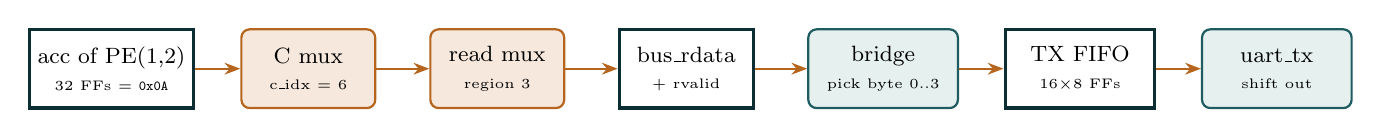
\begin{tikzpicture}[x=1mm,y=1mm]
    \node[seq,  minimum width=19mm, minimum height=10mm] (a) at (0,0)   {acc of PE(1,2)\\\tiny 32 FFs = \hx{0A}};
    \node[comb, minimum width=17mm, minimum height=10mm] (b) at (25,0)  {C mux\\\tiny c\_idx = 6};
    \node[comb, minimum width=17mm, minimum height=10mm] (c) at (49,0)  {read mux\\\tiny region 3};
    \node[seq,  minimum width=17mm, minimum height=10mm] (d) at (73,0)  {bus\_rdata\\\tiny + rvalid};
    \node[mix,  minimum width=19mm, minimum height=10mm] (e) at (98,0)  {bridge\\\tiny pick byte 0..3};
    \node[seq,  minimum width=19mm, minimum height=10mm] (f) at (123,0) {TX FIFO\\\tiny 16$\times$8 FFs};
    \node[mix,  minimum width=19mm, minimum height=10mm] (g) at (148,0) {uart\_tx\\\tiny shift out};
    \foreach \x/\y in {a/b, b/c, c/d, d/e, e/f, f/g} \draw[wire] (\x) -- (\y);
  \end{tikzpicture}}\\[2mm]
  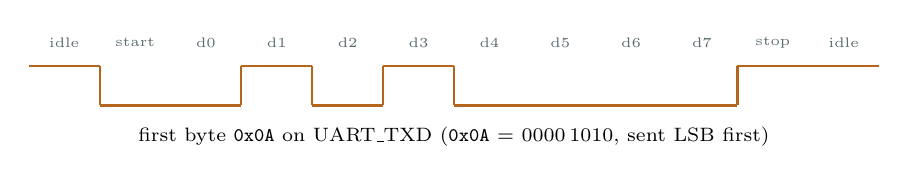
\begin{tikzpicture}[x=1mm,y=1mm]
    \uart{0}{1,0,0,1,0,1,0,0,0,0,1,1}
    \foreach \n/\s in {0/idle, 1/start, 2/d0, 3/d1, 4/d2, 5/d3, 6/d4, 7/d5, 8/d6, 9/d7, 10/stop, 11/idle}
      \node[font=\tiny, text=muted] at (\n*9+4.5,8) {\s};
    \node[font=\scriptsize] at (54,-4) {first byte \hx{0A} on UART\_TXD (\hx{0A} = 0000\,1010, sent LSB first)};
  \end{tikzpicture}

  \vspace{1mm}\raggedright\footnotesize
  \begin{itemize}
    \item The host sends \sig{'D' 00 30 40 00}: read 64 bytes from \hx{3000}. Bytes 24--27 are C[1][2].
          The bridge reads the word at \hx{3018} once per byte and keeps byte (address mod 4): \sig{0A 00 00 00}.
    \item The FIFO is 16 bytes of \textbf{flip-flops} (MAX 10 has no LUT-RAM, and the FIFO reads without a clock edge).
    \item On the PC, NumPy turns \sig{0A 00 00 00} (little-endian int32) into \textbf{10}, which matches A @ B. \checkmark
  \end{itemize}
\end{frame}

% =====================================================================
\begin{frame}{29.\ The time scale: why this design is I/O-bound}
  \centering
  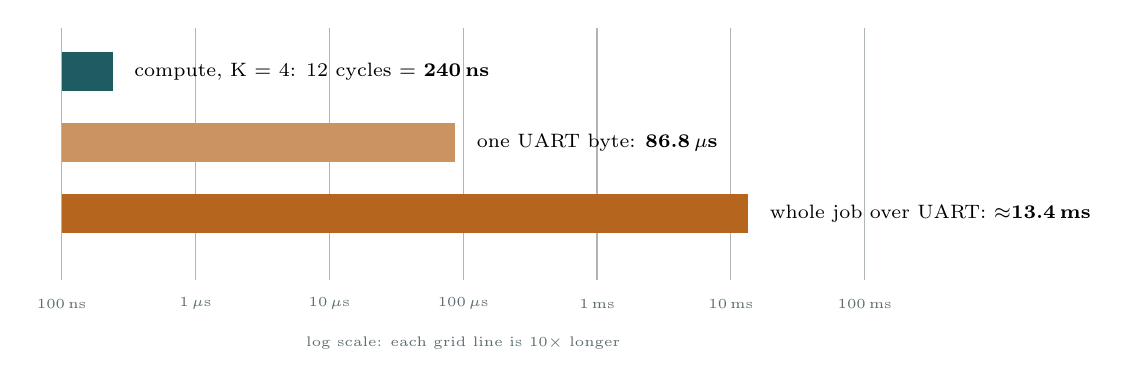
\begin{tikzpicture}[x=1mm,y=1mm]
    \foreach \d/\l in {0/100\,ns, 1/1\,$\mu$s, 2/10\,$\mu$s, 3/100\,$\mu$s, 4/1\,ms, 5/10\,ms, 6/100\,ms} {
      \draw[muted!50] (\d*17,-2) -- (\d*17,30);
      \node[font=\tiny, text=muted] at (\d*17,-5) {\l};
    }
    \fill[pcbmid] (0,22) rectangle (6.5,27);   \node[font=\scriptsize, anchor=west] at (8,24.5) {compute, K = 4: 12 cycles = \textbf{240\,ns}};
    \fill[copper!70] (0,13) rectangle (50,18); \node[font=\scriptsize, anchor=west] at (51.5,15.5) {one UART byte: \textbf{86.8\,$\mu$s}};
    \fill[copper] (0,4) rectangle (87.2,9);    \node[font=\scriptsize, anchor=west] at (88.7,6.5) {whole job over UART: \textbf{$\approx$13.4\,ms}};
    \node[font=\tiny, text=muted] at (51,-10) {log scale: each grid line is 10$\times$ longer};
  \end{tikzpicture}

  \vspace{2mm}\raggedright\small
  \begin{itemize}
    \item Bytes on the wire for one job: 79 to the board (CFG\_K, 4 A rows, B, START, STATUS, read C) + 75 back
          (7 acknowledgements, STATUS, 64 bytes of C) = \textbf{154 bytes} $\times$ 86.8\,$\mu$s $\approx$ 13.4\,ms,
          before USB latency.
    \item 13.4\,ms / 240\,ns $\approx$ \textbf{56\,000$\times$}. The array is idle almost all the time; a faster link
          (not a faster array) is the real next step.
  \end{itemize}
\end{frame}

% =====================================================================
\begin{frame}{30.\ The pattern behind every station}
  \centering
  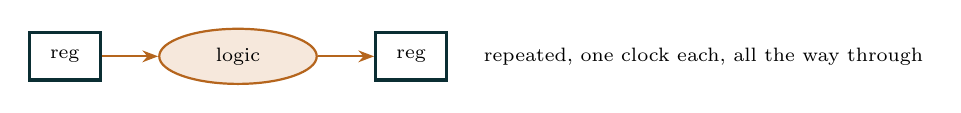
\begin{tikzpicture}[x=1mm,y=1mm]
    \node[seq, minimum width=9mm, minimum height=6mm, font=\scriptsize] (r1) at (0,0) {reg};
    \node[comb, ellipse, minimum width=20mm, minimum height=7mm, font=\scriptsize] (c1) at (22,0) {logic};
    \node[seq, minimum width=9mm, minimum height=6mm, font=\scriptsize] (r2) at (44,0) {reg};
    \draw[wire] (r1) -- (c1); \draw[wire] (c1) -- (r2);
    \node[font=\scriptsize, anchor=west] at (52,0) {repeated, one clock each, all the way through};
  \end{tikzpicture}\\[2mm]
  \footnotesize
  \begin{tabular}{@{}lll@{}}
    \toprule
    \textbf{Register (start)} & \textbf{Logic in between} & \textbf{Register (end)} \\
    \midrule
    \sig{sync\_2ff} output & counter compare, shift select & \sig{shreg} \\
    \sig{uart\_rx.data} & bridge command decode & bridge address / data registers \\
    bridge \sig{bus\_addr} & address decode, bank select, address mux & M9K input registers \\
    M9K address register & RAM read, gate (\sig{rd\_valid}) & skew register (or PE(0,j) \sig{acc}) \\
    skew / \sig{a\_out} register & multiply, sign-extend, add & next PE's \sig{acc} and \sig{a\_out} \\
    \sig{acc} of PE(1,2) & C mux, read mux & \sig{bus\_rdata} \\
    \sig{bus\_rdata} & bridge byte select & FIFO $\rightarrow$ \sig{uart\_tx} shift register $\rightarrow$ pin \\
    \bottomrule
  \end{tabular}\\[2mm]
  \raggedright\small
  If you can draw this for one value, you understand the design. The \textbf{slowest} ``logic in between'' sets the
  maximum clock (Fmax); everything else is just how many clocks it takes.
\end{frame}

% =====================================================================
\section{On the chip}
\begin{frame}{31.\ Timing paths and the 20\,ns budget}
  \begin{columns}[T]
    \column{0.55\textwidth}\small
    Every path is register $\rightarrow$ logic $\rightarrow$ register and must satisfy\\[1mm]
    \centerline{$t_{\text{clk}\rightarrow Q} + t_{\text{logic}} + t_{\text{routing}} + t_{\text{setup}} \le 20$\,ns}
    \vspace{1mm}
    \begin{enumerate}
      \item \textbf{M9K $\rightarrow$ gate $\rightarrow$ PE(0,0) multiply + add $\rightarrow$ acc}: lane 0 has no skew
            register. \textcolor{copper}{\textbf{Likely the slowest.}}
      \item \sig{a\_out} / skew register $\rightarrow$ multiply + add $\rightarrow$ \sig{acc} (every other PE).
      \item \sig{t} $\rightarrow$ compare $\rightarrow$ \sig{state}; \sig{t} $\rightarrow$ address mux $\rightarrow$ M9K.
      \item \sig{acc} $\rightarrow$ 16:1 mux $\rightarrow$ read mux $\rightarrow$ \sig{bus\_rdata}.
      \item bridge registers $\rightarrow$ decode $\rightarrow$ M9K write.
    \end{enumerate}
    \column{0.42\textwidth}\small
    \begin{itemize}
      \item The \textbf{Timing Analyzer} reports the slack of the worst path. Slack $\ge$ 0 means 50\,MHz works.
      \item If path 1 fails: register the gate output (+1 cycle of latency) or pipeline the PE (Lab 9).
      \item The paths through hundreds of PEs are all the same length: \textbf{the array does not get slower as N grows},
            but the C mux does.
      \item None of this is measured yet. It is the first thing to read after the Quartus compile.
    \end{itemize}
  \end{columns}
\end{frame}

% =====================================================================
\begin{frame}{32.\ Estimated resources for the 4$\times$4 build}
  \small
  \resizebox{\textwidth}{!}{%
\begin{tabular}{@{}lrrl@{}}
    \toprule
    \textbf{Block} & \textbf{Flip-flops} & \textbf{LUT logic} & \textbf{Hard blocks} \\
    \midrule
    16 PEs & 704 (768 in RTL) & 512 adder bits (same LEs as \sig{acc}) & 16 multipliers (9$\times$9) \\
    Skew buffers & 96 & --- & --- \\
    RAM banks + gate & 1 (\sig{rd\_valid}) & $\approx$80: select, address mux, gate & 8 M9K \\
    Controller & 17 & $\approx$40 & --- \\
    mm\_regs + 5 counters & 202 & $\approx$250 decode/muxes + 160 counter bits & --- \\
    C readout mux & --- & $\approx$320 & --- \\
    UART, bridge, FIFO, display & $\approx$330 & $\approx$300 & --- \\
    \midrule
    \textbf{Total (rough)} & \textbf{$\approx$1\,350} & \textbf{$\approx$2\,000 LEs ($\approx$4\,\% of 49\,760)} & \textbf{16 / 288, 8 / 182} \\
    \bottomrule
  \end{tabular}}\\[3mm]
  \begin{itemize}
    \item These are \textbf{hand estimates}. The Quartus Fitter report (``Resource Utilization by Entity'') gives the
          real numbers per instance.
    \item The design is small for this chip: the limit for bigger N is the 288 multipliers (16$\times$16 needs 256), not LEs.
  \end{itemize}
\end{frame}

% =====================================================================
\begin{frame}{33.\ From RTL to bits: what Quartus does to the 4$\times$4}
  \small
  \resizebox{\textwidth}{!}{%
\begin{tabular}{@{}p{3.2cm}p{7.8cm}p{3.2cm}@{}}
    \toprule
    \textbf{Step} & \textbf{What happens to our design} & \textbf{Where to look} \\
    \midrule
    Analysis \& Elaboration & 15 files read; \sig{top\_de10lite} found; N = 4 makes 16 PEs, 8 RAMs: 44 instances & Hierarchy tab \\
    Synthesis & \sig{always\_ff} $\rightarrow$ flip-flops; \sig{+} $\rightarrow$ carry chains; \sig{*} $\rightarrow$ multipliers;
                \sig{mem} $\rightarrow$ M9K; \sig{case}/\sig{?:} $\rightarrow$ LUTs; unused edge registers removed & RTL Viewer, Technology Map Viewer \\
    Fitter (place \& route) & LEs packed into LABs; multipliers and M9Ks in their columns; wires routed; pins fixed & Chip Planner, Fitter report \\
    Timing Analyzer & every register-to-register path checked against 20\,ns & slack, Fmax, worst paths \\
    Assembler & configuration bits written to \sig{.sof} & output\_files/ \\
    Programmer & \sig{.sof} sent over the USB-Blaster (JTAG) into the chip & the board runs \\
    \bottomrule
  \end{tabular}}\\[3mm]
  \raggedright
  The hierarchy is flattened for the chip, but the reports keep the instance names, so you can still find
  ``PE(1,2)'' as \sig{g\_row[1].g\_col[2].u\_pe}.
\end{frame}

% =====================================================================
\section{Wrap-up}
\begin{frame}{34.\ Summary: every block, split into its two kinds}
  \footnotesize
  \resizebox{\textwidth}{!}{%
\begin{tabular}{@{}llll@{}}
    \toprule
    \textbf{Block} & \textbf{Sequential (flip-flops)} & \textbf{Combinational (logic)} & \textbf{Hard block} \\
    \midrule
    PE & \sig{acc}, \sig{a\_out}, \sig{b\_out} & 32-bit adder; sign extension = wires & 9$\times$9 multiplier \\
    Array & (the PE registers) & none: only wires between PEs & --- \\
    Skew buffer & 6 registers per buffer & none (lane 0 is a wire) & --- \\
    RAM banks & \sig{rd\_valid} & bank select, address mux & M9K (registered address) \\
    Gate & --- & 32 AND per side & --- \\
    Controller & \sig{state}, \sig{t}, \sig{k\_r} & next-state, $t+1$, compares, output decode & --- \\
    mm\_regs & config, flags, 5 counters, \sig{bus\_rdata} & address decode, read mux, counter adders & --- \\
    C readout & --- & 16:1 $\times$ 32 multiplexer & --- \\
    UART RX / TX & synchronizer, counters, shift registers, FSM & compares, next-state & --- \\
    TX FIFO & 16 $\times$ 8 storage, pointers & read mux, full/empty & --- \\
    \bottomrule
  \end{tabular}}\\[3mm]
  \small
  \textbf{Takeaway:} the systolic array is mostly \emph{sequential} (registers everywhere) with small, identical
  combinational pieces in between. That regularity is what makes it fast and easy to place on an FPGA.
\end{frame}

% =====================================================================
\begin{frame}{35.\ Check yourself}
  \small
  \begin{enumerate}
    \item Which parts of a PE are combinational, which are sequential, and which are hard blocks?
    \item Why is there a \sig{rd\_valid} register?
    \item Why does the gate force zeros? What would go wrong without it?
    \item At which step does $A[2][1]$ reach PE(2,3)?
    \item How many flip-flops are in the two skew buffers for N = 4, and why?
    \item At which address is $B[3][1]$? Which bank and which RAM address hold it?
    \item Why must N and K\_MAX be powers of 2?
    \item Why should Quartus keep only 704 of the 768 PE flip-flops?
    \item What is the likely critical path, and how would you fix it if 20\,ns is not met?
    \item For K = 4: how many cycles, and what PE utilization?
  \end{enumerate}
\end{frame}

% =====================================================================
\begin{frame}{36.\ Answers}
  \footnotesize
  \begin{enumerate}
    \item Combinational: adder (sign extension is wires). Sequential: \sig{acc}, \sig{a\_out}, \sig{b\_out}.
          Hard: the 9$\times$9 multiplier.
    \item The M9K returns data one clock after the address. \sig{rd\_valid} is \sig{rd\_en} delayed one clock, so it lines up with the data.
    \item The RAM reads every cycle; outside the K valid reads it shows old data. Without zeros the PEs would add garbage.
    \item $t = k + 1 + i + j = 1 + 1 + 2 + 3 = \mathbf{7}$.
    \item $2 \times (0+1+2+3) \times 8 = \mathbf{96}$: lane $n$ needs $n$ registers of 8 bits.
    \item \hx{2000} + 4$\cdot$3 + 1 = \hx{200D}: bank B1, RAM address 3.
    \item Then ``divide by 64'' and ``mod 64'' are bit slices (free wires). Other sizes need divide logic.
    \item The last column's \sig{a\_out} and the bottom row's \sig{b\_out} drive nothing: $8 \times 8 = 64$ flip-flops are removed.
    \item M9K $\rightarrow$ gate $\rightarrow$ PE(0,0) multiply + add $\rightarrow$ acc. Register the gate output, or pipeline the PE.
    \item 12 cycles (= K + 2N); utilization $64 / (16 \times 11) = 36\,\%$.
  \end{enumerate}
\end{frame}

\end{document}
